% Options for packages loaded elsewhere
\PassOptionsToPackage{unicode}{hyperref}
\PassOptionsToPackage{hyphens}{url}
\PassOptionsToPackage{dvipsnames,svgnames,x11names}{xcolor}
%
\documentclass[
  letterpaper,
  DIV=11,
  numbers=noendperiod]{scrartcl}

\usepackage{amsmath,amssymb}
\usepackage{setspace}
\usepackage{iftex}
\ifPDFTeX
  \usepackage[T1]{fontenc}
  \usepackage[utf8]{inputenc}
  \usepackage{textcomp} % provide euro and other symbols
\else % if luatex or xetex
  \usepackage{unicode-math}
  \defaultfontfeatures{Scale=MatchLowercase}
  \defaultfontfeatures[\rmfamily]{Ligatures=TeX,Scale=1}
\fi
\usepackage{lmodern}
\ifPDFTeX\else  
    % xetex/luatex font selection
\fi
% Use upquote if available, for straight quotes in verbatim environments
\IfFileExists{upquote.sty}{\usepackage{upquote}}{}
\IfFileExists{microtype.sty}{% use microtype if available
  \usepackage[]{microtype}
  \UseMicrotypeSet[protrusion]{basicmath} % disable protrusion for tt fonts
}{}
\makeatletter
\@ifundefined{KOMAClassName}{% if non-KOMA class
  \IfFileExists{parskip.sty}{%
    \usepackage{parskip}
  }{% else
    \setlength{\parindent}{0pt}
    \setlength{\parskip}{6pt plus 2pt minus 1pt}}
}{% if KOMA class
  \KOMAoptions{parskip=half}}
\makeatother
\usepackage{xcolor}
\usepackage[top=1in,bottom=1in,left=1.5in,right=1in]{geometry}
\setlength{\emergencystretch}{3em} % prevent overfull lines
\setcounter{secnumdepth}{-\maxdimen} % remove section numbering
% Make \paragraph and \subparagraph free-standing
\makeatletter
\ifx\paragraph\undefined\else
  \let\oldparagraph\paragraph
  \renewcommand{\paragraph}{
    \@ifstar
      \xxxParagraphStar
      \xxxParagraphNoStar
  }
  \newcommand{\xxxParagraphStar}[1]{\oldparagraph*{#1}\mbox{}}
  \newcommand{\xxxParagraphNoStar}[1]{\oldparagraph{#1}\mbox{}}
\fi
\ifx\subparagraph\undefined\else
  \let\oldsubparagraph\subparagraph
  \renewcommand{\subparagraph}{
    \@ifstar
      \xxxSubParagraphStar
      \xxxSubParagraphNoStar
  }
  \newcommand{\xxxSubParagraphStar}[1]{\oldsubparagraph*{#1}\mbox{}}
  \newcommand{\xxxSubParagraphNoStar}[1]{\oldsubparagraph{#1}\mbox{}}
\fi
\makeatother


\providecommand{\tightlist}{%
  \setlength{\itemsep}{0pt}\setlength{\parskip}{0pt}}\usepackage{longtable,booktabs,array}
\usepackage{calc} % for calculating minipage widths
% Correct order of tables after \paragraph or \subparagraph
\usepackage{etoolbox}
\makeatletter
\patchcmd\longtable{\par}{\if@noskipsec\mbox{}\fi\par}{}{}
\makeatother
% Allow footnotes in longtable head/foot
\IfFileExists{footnotehyper.sty}{\usepackage{footnotehyper}}{\usepackage{footnote}}
\makesavenoteenv{longtable}
\usepackage{graphicx}
\makeatletter
\def\maxwidth{\ifdim\Gin@nat@width>\linewidth\linewidth\else\Gin@nat@width\fi}
\def\maxheight{\ifdim\Gin@nat@height>\textheight\textheight\else\Gin@nat@height\fi}
\makeatother
% Scale images if necessary, so that they will not overflow the page
% margins by default, and it is still possible to overwrite the defaults
% using explicit options in \includegraphics[width, height, ...]{}
\setkeys{Gin}{width=\maxwidth,height=\maxheight,keepaspectratio}
% Set default figure placement to htbp
\makeatletter
\def\fps@figure{htbp}
\makeatother
% definitions for citeproc citations
\NewDocumentCommand\citeproctext{}{}
\NewDocumentCommand\citeproc{mm}{%
  \begingroup\def\citeproctext{#2}\cite{#1}\endgroup}
\makeatletter
 % allow citations to break across lines
 \let\@cite@ofmt\@firstofone
 % avoid brackets around text for \cite:
 \def\@biblabel#1{}
 \def\@cite#1#2{{#1\if@tempswa , #2\fi}}
\makeatother
\newlength{\cslhangindent}
\setlength{\cslhangindent}{1.5em}
\newlength{\csllabelwidth}
\setlength{\csllabelwidth}{3em}
\newenvironment{CSLReferences}[2] % #1 hanging-indent, #2 entry-spacing
 {\begin{list}{}{%
  \setlength{\itemindent}{0pt}
  \setlength{\leftmargin}{0pt}
  \setlength{\parsep}{0pt}
  % turn on hanging indent if param 1 is 1
  \ifodd #1
   \setlength{\leftmargin}{\cslhangindent}
   \setlength{\itemindent}{-1\cslhangindent}
  \fi
  % set entry spacing
  \setlength{\itemsep}{#2\baselineskip}}}
 {\end{list}}
\usepackage{calc}
\newcommand{\CSLBlock}[1]{\hfill\break\parbox[t]{\linewidth}{\strut\ignorespaces#1\strut}}
\newcommand{\CSLLeftMargin}[1]{\parbox[t]{\csllabelwidth}{\strut#1\strut}}
\newcommand{\CSLRightInline}[1]{\parbox[t]{\linewidth - \csllabelwidth}{\strut#1\strut}}
\newcommand{\CSLIndent}[1]{\hspace{\cslhangindent}#1}

\usepackage{booktabs}
\usepackage{longtable}
\usepackage{array}
\usepackage{multirow}
\usepackage{wrapfig}
\usepackage{float}
\usepackage{colortbl}
\usepackage{pdflscape}
\usepackage{tabu}
\usepackage{threeparttable}
\usepackage{threeparttablex}
\usepackage[normalem]{ulem}
\usepackage{makecell}
\usepackage{xcolor}
\usepackage{lineno}\linenumbers
\KOMAoption{captions}{tableheading}
\makeatletter
\@ifpackageloaded{tcolorbox}{}{\usepackage[skins,breakable]{tcolorbox}}
\@ifpackageloaded{fontawesome5}{}{\usepackage{fontawesome5}}
\definecolor{quarto-callout-color}{HTML}{909090}
\definecolor{quarto-callout-note-color}{HTML}{0758E5}
\definecolor{quarto-callout-important-color}{HTML}{CC1914}
\definecolor{quarto-callout-warning-color}{HTML}{EB9113}
\definecolor{quarto-callout-tip-color}{HTML}{00A047}
\definecolor{quarto-callout-caution-color}{HTML}{FC5300}
\definecolor{quarto-callout-color-frame}{HTML}{acacac}
\definecolor{quarto-callout-note-color-frame}{HTML}{4582ec}
\definecolor{quarto-callout-important-color-frame}{HTML}{d9534f}
\definecolor{quarto-callout-warning-color-frame}{HTML}{f0ad4e}
\definecolor{quarto-callout-tip-color-frame}{HTML}{02b875}
\definecolor{quarto-callout-caution-color-frame}{HTML}{fd7e14}
\makeatother
\makeatletter
\@ifpackageloaded{caption}{}{\usepackage{caption}}
\AtBeginDocument{%
\ifdefined\contentsname
  \renewcommand*\contentsname{Table of contents}
\else
  \newcommand\contentsname{Table of contents}
\fi
\ifdefined\listfigurename
  \renewcommand*\listfigurename{List of Figures}
\else
  \newcommand\listfigurename{List of Figures}
\fi
\ifdefined\listtablename
  \renewcommand*\listtablename{List of Tables}
\else
  \newcommand\listtablename{List of Tables}
\fi
\ifdefined\figurename
  \renewcommand*\figurename{Figure}
\else
  \newcommand\figurename{Figure}
\fi
\ifdefined\tablename
  \renewcommand*\tablename{Table}
\else
  \newcommand\tablename{Table}
\fi
}
\@ifpackageloaded{float}{}{\usepackage{float}}
\floatstyle{ruled}
\@ifundefined{c@chapter}{\newfloat{codelisting}{h}{lop}}{\newfloat{codelisting}{h}{lop}[chapter]}
\floatname{codelisting}{Listing}
\newcommand*\listoflistings{\listof{codelisting}{List of Listings}}
\makeatother
\makeatletter
\makeatother
\makeatletter
\@ifpackageloaded{caption}{}{\usepackage{caption}}
\@ifpackageloaded{subcaption}{}{\usepackage{subcaption}}
\makeatother

\ifLuaTeX
  \usepackage{selnolig}  % disable illegal ligatures
\fi
\usepackage{bookmark}

\IfFileExists{xurl.sty}{\usepackage{xurl}}{} % add URL line breaks if available
\urlstyle{same} % disable monospaced font for URLs
\hypersetup{
  pdftitle={Chapter 3},
  pdfauthor={Tyler Wiederich},
  colorlinks=true,
  linkcolor={blue},
  filecolor={Maroon},
  citecolor={Blue},
  urlcolor={Blue},
  pdfcreator={LaTeX via pandoc}}


\title{Chapter 3}
\author{Tyler Wiederich}
\date{March 23, 2026}

\begin{document}
\maketitle
\begin{abstract}
The display of 3-dimensional (3D) data is often limited by how it can be
rendered. These renderings are typically presented as charts on
2-dimensional (2D) computer screens using 2D or 3D chart styles.
However, computer renderings do not provide the level of interactivity
of 3D charts that we experience in a 3D world, something which can be
accomplished through the use of 3D printing. In this paper, we describe
a study to compare 2D and 3D heatmaps rendered digitally or via 3D
printing and assess the findings of 3D printed charts for the use of
displaying statistical information.
\end{abstract}


\setstretch{2}
\subsection{Introduction}\label{introduction}

In the 20th century, advancements in technology made data visualizations
increasingly more affordable and accessible to a broader population. The
primary change in formal data visualizations was from hand-drawn charts
to computer-rendered charts (Tukey 1965), and with subsequent advances
in color printing and available software have allowed for data
visualizations to enter other mediums. These include the ability create
virtual and physical charts that effectively use the 3-dimensional (3D)
world around us with the novel use of 3D-printed charts. This newer type
of visualization has gained a small amount of traction in recent years
as a method of producing tangible charts (Stusak, Hobe, and Butz 2016;
Hu 2015; Huron et al. 2023).

In many disciplines, 3D-printed visualizations have shown mixed or
promising results compared to alternative rendering formats. Although a
comprehensive review of 3D-printing in scientific fields is beyond the
scope of this paper, we highlight several examples of its use for
visualization. Katsioloudis and Jones (2018) conducted a study with
engineering students and found no statistically significant difference
between computer-rendered and 3D-printed models when students were asked
to draw a cross-section of a dodecahedron, suggesting similar levels of
spatial understanding between digital and physical representations. In
contrast, other applications have highlighted advantages of 3D-printed
models. For example, Holloway et al. (2019) reported positive feedback
from visually impaired individuals when 3D-printed maps were used to
support navigation. Similarly, in clinical education, Muff et al. (2022)
found that 3D-printed anatomical structures were well accepted alongside
VR glasses and 3D computer renderings. As 3D-printed visualizations
become increasingly common across scientific fields, we explore their
potential use in communicating statistical graphics.

At this time, there are few studies that evaluate 3D-printed charts for
the purpose of displaying statistical information (Jansen, Dragicevic,
and Fekete 2013; Stusak, Schwarz, and Butz 2015; Stusak, Hobe, and Butz
2016; Hu 2015). This may in part be due to the cost of materials and
rendering times as compared to charts produced on a computer. A single
chart can take up to a day to print, limiting the ability to quickly
produce visualizations. Additionally, there are few options for
producing such charts from statistical software. In R, the \texttt{rgl}
package (Murdoch and Adler 2023) can export STL files that can be used
by 3D-printing software, and similarly for the \texttt{rayshader}
package (Morgan-Wall 2024). However, these options are not optimized for
essential considerations required of 3D-printed charts, such as embossed
labels. Given the nature of 3-dimensional data, viewing a 3D realization
of statistical information in a 3D environment is a realistic scenario
that could increase the ability for information extraction.

\subsubsection{Literature Review}\label{literature-review}

Using an identical dataset across multiple chart types does not ensure
that the data is perceived in the same way (Cleveland and McGill 1984;
Hofmann et al. 2012; Vanderplas, Cook, and Hofmann 2020). One of the
main factors in this phenomenon is how data is encoded into the chart.
These encodings include, but are not limited to, placement along axes,
lengths, areas, volumes, and color scales. For example, bar charts and
pie charts are two common visualizations that have long been the topic
of debate (Eells 1926; Croxton and Stryker 1927; Cleveland and McGill
1984; Lewandowsky and Spence 1989). Bar charts are constructed with the
encodings of length, position, and area. In contrast, pie charts make
use of arc lengths, angles, and area. Inherently, the comparison of
different chart types is a comparison of encodings due to the changes in
how data is being displayed.

Cleveland and McGill (1984) noted that estimates involving numerical
accuracy may decrease when increasing dimensionality of the encoding,
although this was not formally tested in their experiments. Their
reasoning was due to Stevens' power law, a mathematical formulation of
how magnitudes are perceived given different stimuli sources (Stevens
and Stevens 1986). The general form of the law is \(\psi(I)=kI^\alpha\),
where \(I\) is the magnitude of a stimulus, \(\psi(I)\) is the perceived
magnitude, \(k\) is a proportionality constant from the unit of the
stimulus, and \(\alpha\) is the exponent from the type of stimuli used.
Studies have estimated that lengths are perceived without bias (i.e.,
\(\alpha=1\)), but areas and volumes tend to have skewed perceptions
(Cleveland and McGill 1984). This indicates that lower-dimensional
charts may perform better when readers are tasked with extracting
numerical estimates from the chart, although this has been a topic of
debate in the last several decades.

There are mixed results in regard to the use of 3D charts, mostly
attributable to the use of the third dimension. When the extra dimension
does not convey meaningful information, estimates of accuracy decrease
and solution times increase as compared to equivalent 2D charts (Fisher,
Dempsey, and Marousky 1997; Zacks et al. 1998; Fischer 2000). The same
increase in solution time is seen when the third dimension is utilized
for displaying data, but can sometimes produce better error rates than
2D charts (Barfield and Robless 1989; Kraus et al. 2020). Additionally,
when given the option of 2D or 3D charts for extracting numerical
information, the 2D charts showed increased preference and confidence
than their 3D counterparts (Barfield and Robless 1989; Fisher, Dempsey,
and Marousky 1997). It is worth noting that all of these studies use 2D
or virtual reality renderings of 3D charts and not physical 3D charts.

Many studies that assess 3D charts use computer-rendered displays that
leverage high levels of precision in their output. Digital renderings
allow for exact control over visual properties, whereas physical charts
are subject to factors such as chart materials, lighting conditions,
interactivity, and viewing distance. Some of these factors have already
been suggested to have a measureable effect within computer renderings
(Tarr and Kriegman 2001; Wang et al. 2022). While virtual reality can
offer similar interactions with 3D objects compared to the real world,
perceptual judgements can be distorted in virtual environments
(\textbf{kelly2018?}; \textbf{park2021?}). The result is that many
findings for the perception of 3D statistical graphics are limited to
the method in which they were rendered.

To date, few empirical studies have investigated 3D-printed charts, and
it is unclear if they follow the framework of existing theories on data
visualizations. One of the first studies to examine digital and physical
renderings primarily focused on information retrieval times, where
physical 3D heatmaps had lower completion times than digitized 2D and 3D
alternatives (Jansen, Dragicevic, and Fekete 2013). In their study,
error rates were also collected, but had small effect sizes due to the
2D, digital 3D, and physical 3D charts. Other studies on physical
statistical graphics tend to focus on bar charts, where the third
dimension is not used for information. Physical 3D bar charts are
suggested to have conditionally improved memorability, subject to
specific datasets (Stusak, Schwarz, and Butz 2015; Stusak, Hobe, and
Butz 2016). Hu (2015) discussed the construction of 3D-printed bar
charts with accessibility features, though these designs do not appear
to have been empirically evaluated.

We hypothesize that 3D charts in 3D environments will produce better
information extraction than their computer-rendered counterparts.
Specifically, we compare 3D-printed charts to digital renderings of 2D
static charts and 3D interactive charts. We suspect that this difference
will hold across multiple data sets and different magnitudes of stimuli.
In this paper, we evaluate the accuracy of numerical estimations on true
3D charts by conducting a factorial experiment that assessed chart types
and ratios of pairs of stimuli. We discuss the construction of the
stimuli and how we closely matched the charts to compare 2D, 3D-digital,
and 3D-printed renderings of heatmap data.

\subsection{Methods}\label{methods}

Our study was designed to evaluate and expand the literature on
numerical estimation of dimensionality for 3D charts. In our study, we
focused on 2D and 3D heatmaps, which we carefully constructed to ensure
that differences can be attributed to the dimensionality of the chart
and the mapping of data when comparing 2D to 3D. All of our data and
methods are publicly available for open science and reproducibility at
\url{https://github.com/TWiedRW/ch3-heat3d}. In this section, we discuss
the process of designing our experiment and participant recruitment.

\subsubsection{Stimuli}\label{stimuli}

We define stimuli as the magnitude of our selected values. In a 3D
Cartesian space, the X- and Y- axes represent the coordinates of the
stimuli, and the Z-axis represents the value for the stimuli. Each X and
Y coordinate is represented by a square tile with a 1:1 aspect ratio. In
a 2D space, the Z variable is mapped to fill with a monochromatic
gradient. All stimuli and remaining randomly generated values range
between 0 and 100 units. In this experiment, \(X=1, 2, \dots,10\) and
\(Y=1, 2,\dots,10\).

Our experiment is designed using the method of constant stimuli, where
comparisons between stimuli are with respect to a stimulus that remains
the same magnitude (Kingdom and Prins 2016, chap. 3). We set the
constant stimuli at 50 units. For stimuli between 50 and 100, we set the
maximum stimuli value at 90 and equally partitioned the ratios of
stimuli with the constant stimuli, \(\frac{50}{90}=0.556\) to
\(\frac{50}{50}=1.0\), resulting in 4 varying stimuli values where 50 is
the smallest value. The same ratios obtained with stimuli between 50 and
90 were used to create 4 stimuli varying between 0 and 50, where 50 is
the largest value. Additionally, we also included a stimulus pair where
both values are 50, resulting in nine total pairs of stimuli. All
stimuli values can be found in Figure~\ref{fig-stimuli-values}.

\begin{figure}

\centering{


\includegraphics{index_files/figure-pdf/fig-stimuli-values-1.pdf}

}

\caption{\label{fig-stimuli-values}Values for stimuli in the heatmap
experiment. All values are paired with the constant stimuli of 50 units,
creating nine pairs of stimuli.}

\end{figure}%

Two datasets were created for the experiment. To generate non-stimuli
random values, we used a mixture distribution of random uniform noise
and a mathematical function to populate our coordinate grid. The
mathematical functions are scaled between 0 and 100,
\(g(Z)=100\cdot\frac{Z-\min(Z)}{\max(Z)-min(Z)}\). The first dataset,
set 1, used the formula for the top half of a sphere that is centered
within our X and Y coordinate grid,
\(f_1(X,Y)=\sqrt{7^2-(X-\bar{X})^2-(Y-\bar{Y})^2}\), where \(\bar{X}\)
and \(\bar{Y}\) are the averages of the \(X\) and \(Y\) coordinate
ranges. The second dataset is calculated similarly using the formula for
the bottom half of a sphere,
\(f_2(X,Y)=\sqrt{7^2-(X-\bar{X})^2+(Y-\bar{Y})^2}\). Denoting \(Z\) as
the random values, \(U(0,100)\) as a random variable drawn from a
continuous uniform distribution between 0 and 100, and \(X,Y\) as
heatmap coordinates, our random heatmap data is calculated in
Equation~\ref{eq-random-z} with \(c=0.3\). An example of varying \(c\)
values is presented in Figure~\ref{fig-random-z}.

\begin{equation}\phantomsection\label{eq-random-z}{
Z=c\cdot U(0,100)+(1-c)\cdot g(f_i(X,Y))
}\end{equation}

\begin{figure}

\begin{minipage}{0.20\linewidth}

\centering{

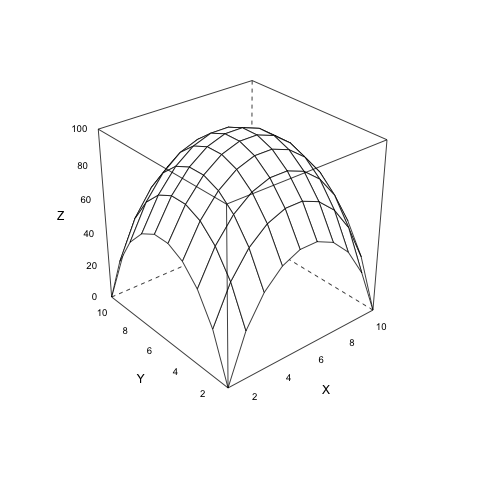
\includegraphics{plots/z100.png}

}

\subcaption{\label{fig-z100}\(c=0\)}

\end{minipage}%
%
\begin{minipage}{0.20\linewidth}

\centering{

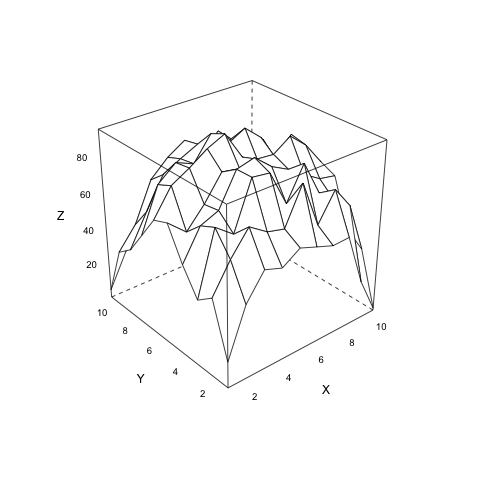
\includegraphics{plots/z75.png}

}

\subcaption{\label{fig-z75}\(c=0.25\)}

\end{minipage}%
%
\begin{minipage}{0.20\linewidth}

\centering{

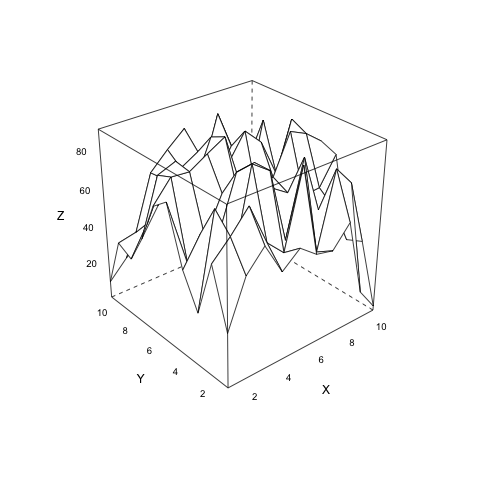
\includegraphics{plots/z50.png}

}

\subcaption{\label{fig-z50}\(c=0.5\)}

\end{minipage}%
%
\begin{minipage}{0.20\linewidth}

\centering{

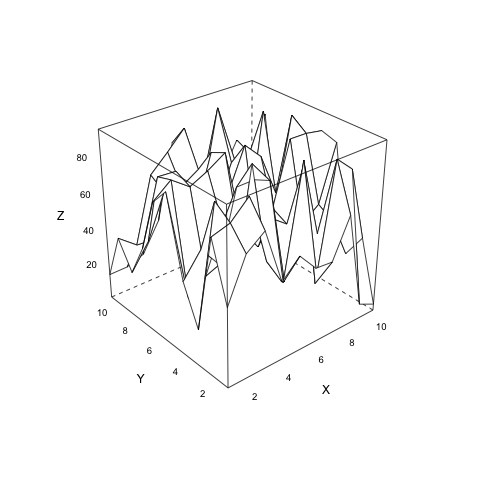
\includegraphics{plots/z25.png}

}

\subcaption{\label{fig-z25}\(c=0.75\)}

\end{minipage}%
%
\begin{minipage}{0.20\linewidth}

\centering{

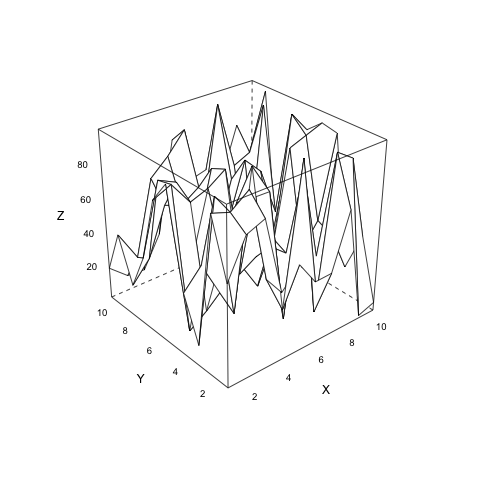
\includegraphics{plots/z0.png}

}

\subcaption{\label{fig-z0}\(c=1\)}

\end{minipage}%

\caption{\label{fig-random-z}Mixture distribution of
Equation~\ref{eq-random-z} using the formula for the top half of a
sphere. As \(c\) approaches 1, the distribution resembles uniform random
noise.}

\end{figure}%

The placement of stimuli values onto the randomly generated heatmap data
was done via simulation to try to make their placement look as natural
as possible. Twenty random heatmaps were generated. For each heatmap,
the non-constant stimuli was placed onto the coordinate such that the
difference between the stimuli and randomly generated value is
minimized. The constant stimuli was then placed onto a coordinate within
a Manhattan distance of three or four that minimizes the difference
between the constant stimuli and randomly generated values, where the
Manhattan distance is given by \(|X_i - X_j| + |Y_i - Y_j|\) for stimuli
\(i\) and \(j\). To ensure that stimuli placement is evenly positioned
across the heatmap, the count of stimuli was computed separately across
the X and Y axes. For example, in Data Set 1, the X-axis has four
stimuli in \(X=1\), three stimuli in \(X=2\), and so forth. Chi-squared
statistics were calculated for each axis and the heatmap with the
smallest average Chi-squared statistic was selected as the final
dataset. A visual inspection of this process showed that the stimuli
were not clustered in any one area of the chart and that the stimuli
look natural with respect to the random mixture distribution.

\begin{figure}

\begin{minipage}{0.50\linewidth}

\centering{

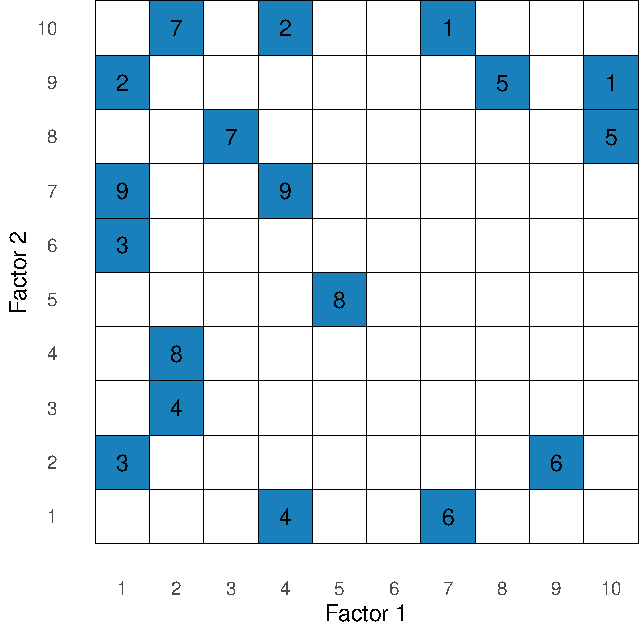
\includegraphics[width=0.95\textwidth,height=\textheight]{index_files/figure-pdf/fig-placement-1.pdf}

}

\subcaption{\label{fig-placement-1}Placement of stimuli on Set 1}

\end{minipage}%
%
\begin{minipage}{0.50\linewidth}

\centering{

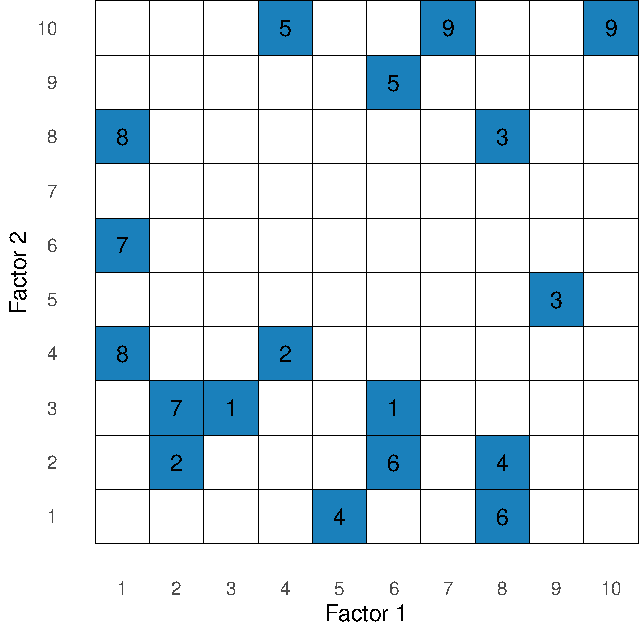
\includegraphics[width=0.95\textwidth,height=\textheight]{index_files/figure-pdf/fig-placement-2.pdf}

}

\subcaption{\label{fig-placement-2}Placement of stimuli on Set 2}

\end{minipage}%

\caption{\label{fig-placement}Placement of stimuli on the two data sets.
Tiles with solid fills are the fixed stimuli values, where white tiles
are randomly generated.}

\end{figure}%

\subsubsection{Charts}\label{charts}

Three types of charts were considered for this study: digital and static
2D (2dd), digital and interactive 3D (3dd), and 3D-printed (3dp). We
constructed these charts so that they were as similar as possible, but
inherent differences in dimensionality led to artistic decisions that
attempt to focus solely on the dimensionality of the charts. The process
of creating the charts is discussed in this section.

The 3D-printed charts were rendered with OpenSCAD (Kintel 2023). To
include plot text, a 120mm by 120mm by 10mm base was created with a
solid color that was either white or black. Cells of the heatmap
measured 10mm by 10mm, resulting in a heatmap that is 100mm by 100mm and
is centered on the base. The upper bound of the height of heatmap values
is 100mm, where 1-unit in the heatmap data is represented by 1mm of
height on the heatmap. Once rendered, the heatmap was saved to 3D
Manufacturing Format (3mf) and Standard Triangle Language (stl) files. A
variety of solid and gradient filaments were tested for the bars of the
3D prints, and we eventually settled on a rainbow gradient. Some charts
were printed with a white base and black text, and other charts had a
black base with white text. An example of the 3D-printed chart is shown
in Figure~\ref{fig-3dp}.

\begin{figure}

\begin{minipage}{0.50\linewidth}

\centering{

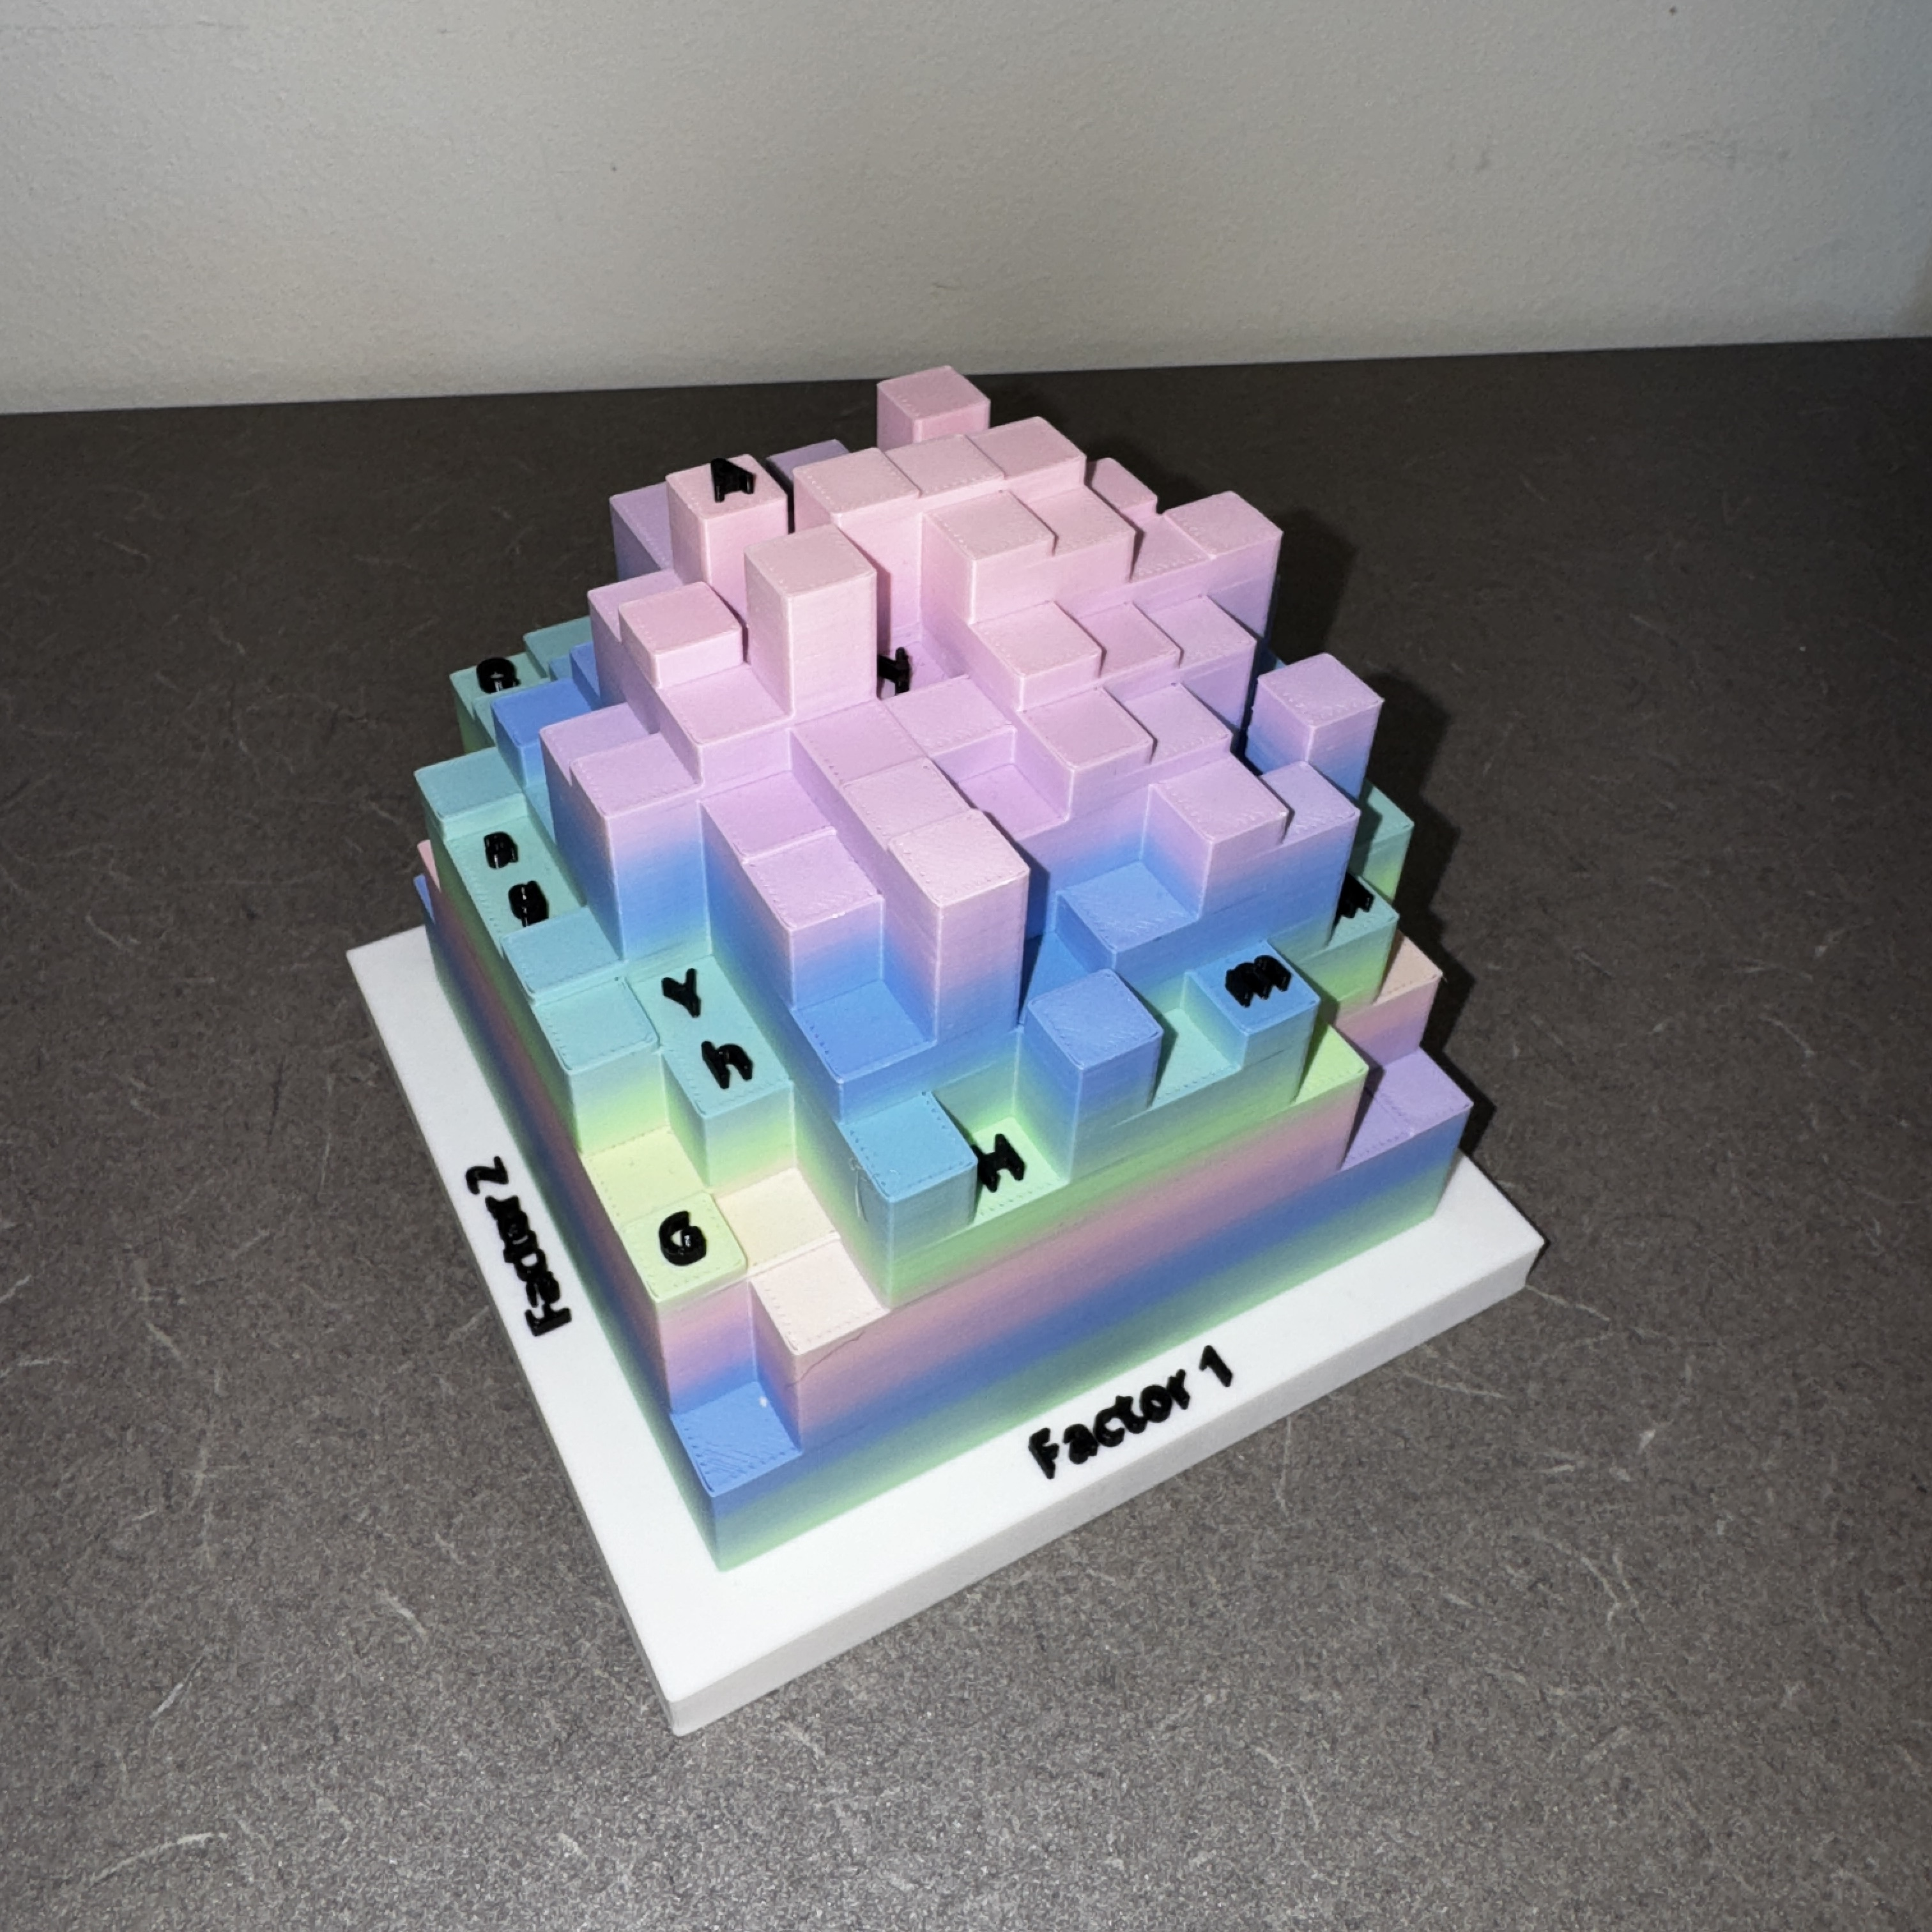
\includegraphics{images/3dp-gradient-set1.JPG}

}

\subcaption{\label{fig-3dp-gradient}Data Set 1}

\end{minipage}%
%
\begin{minipage}{0.50\linewidth}

\centering{

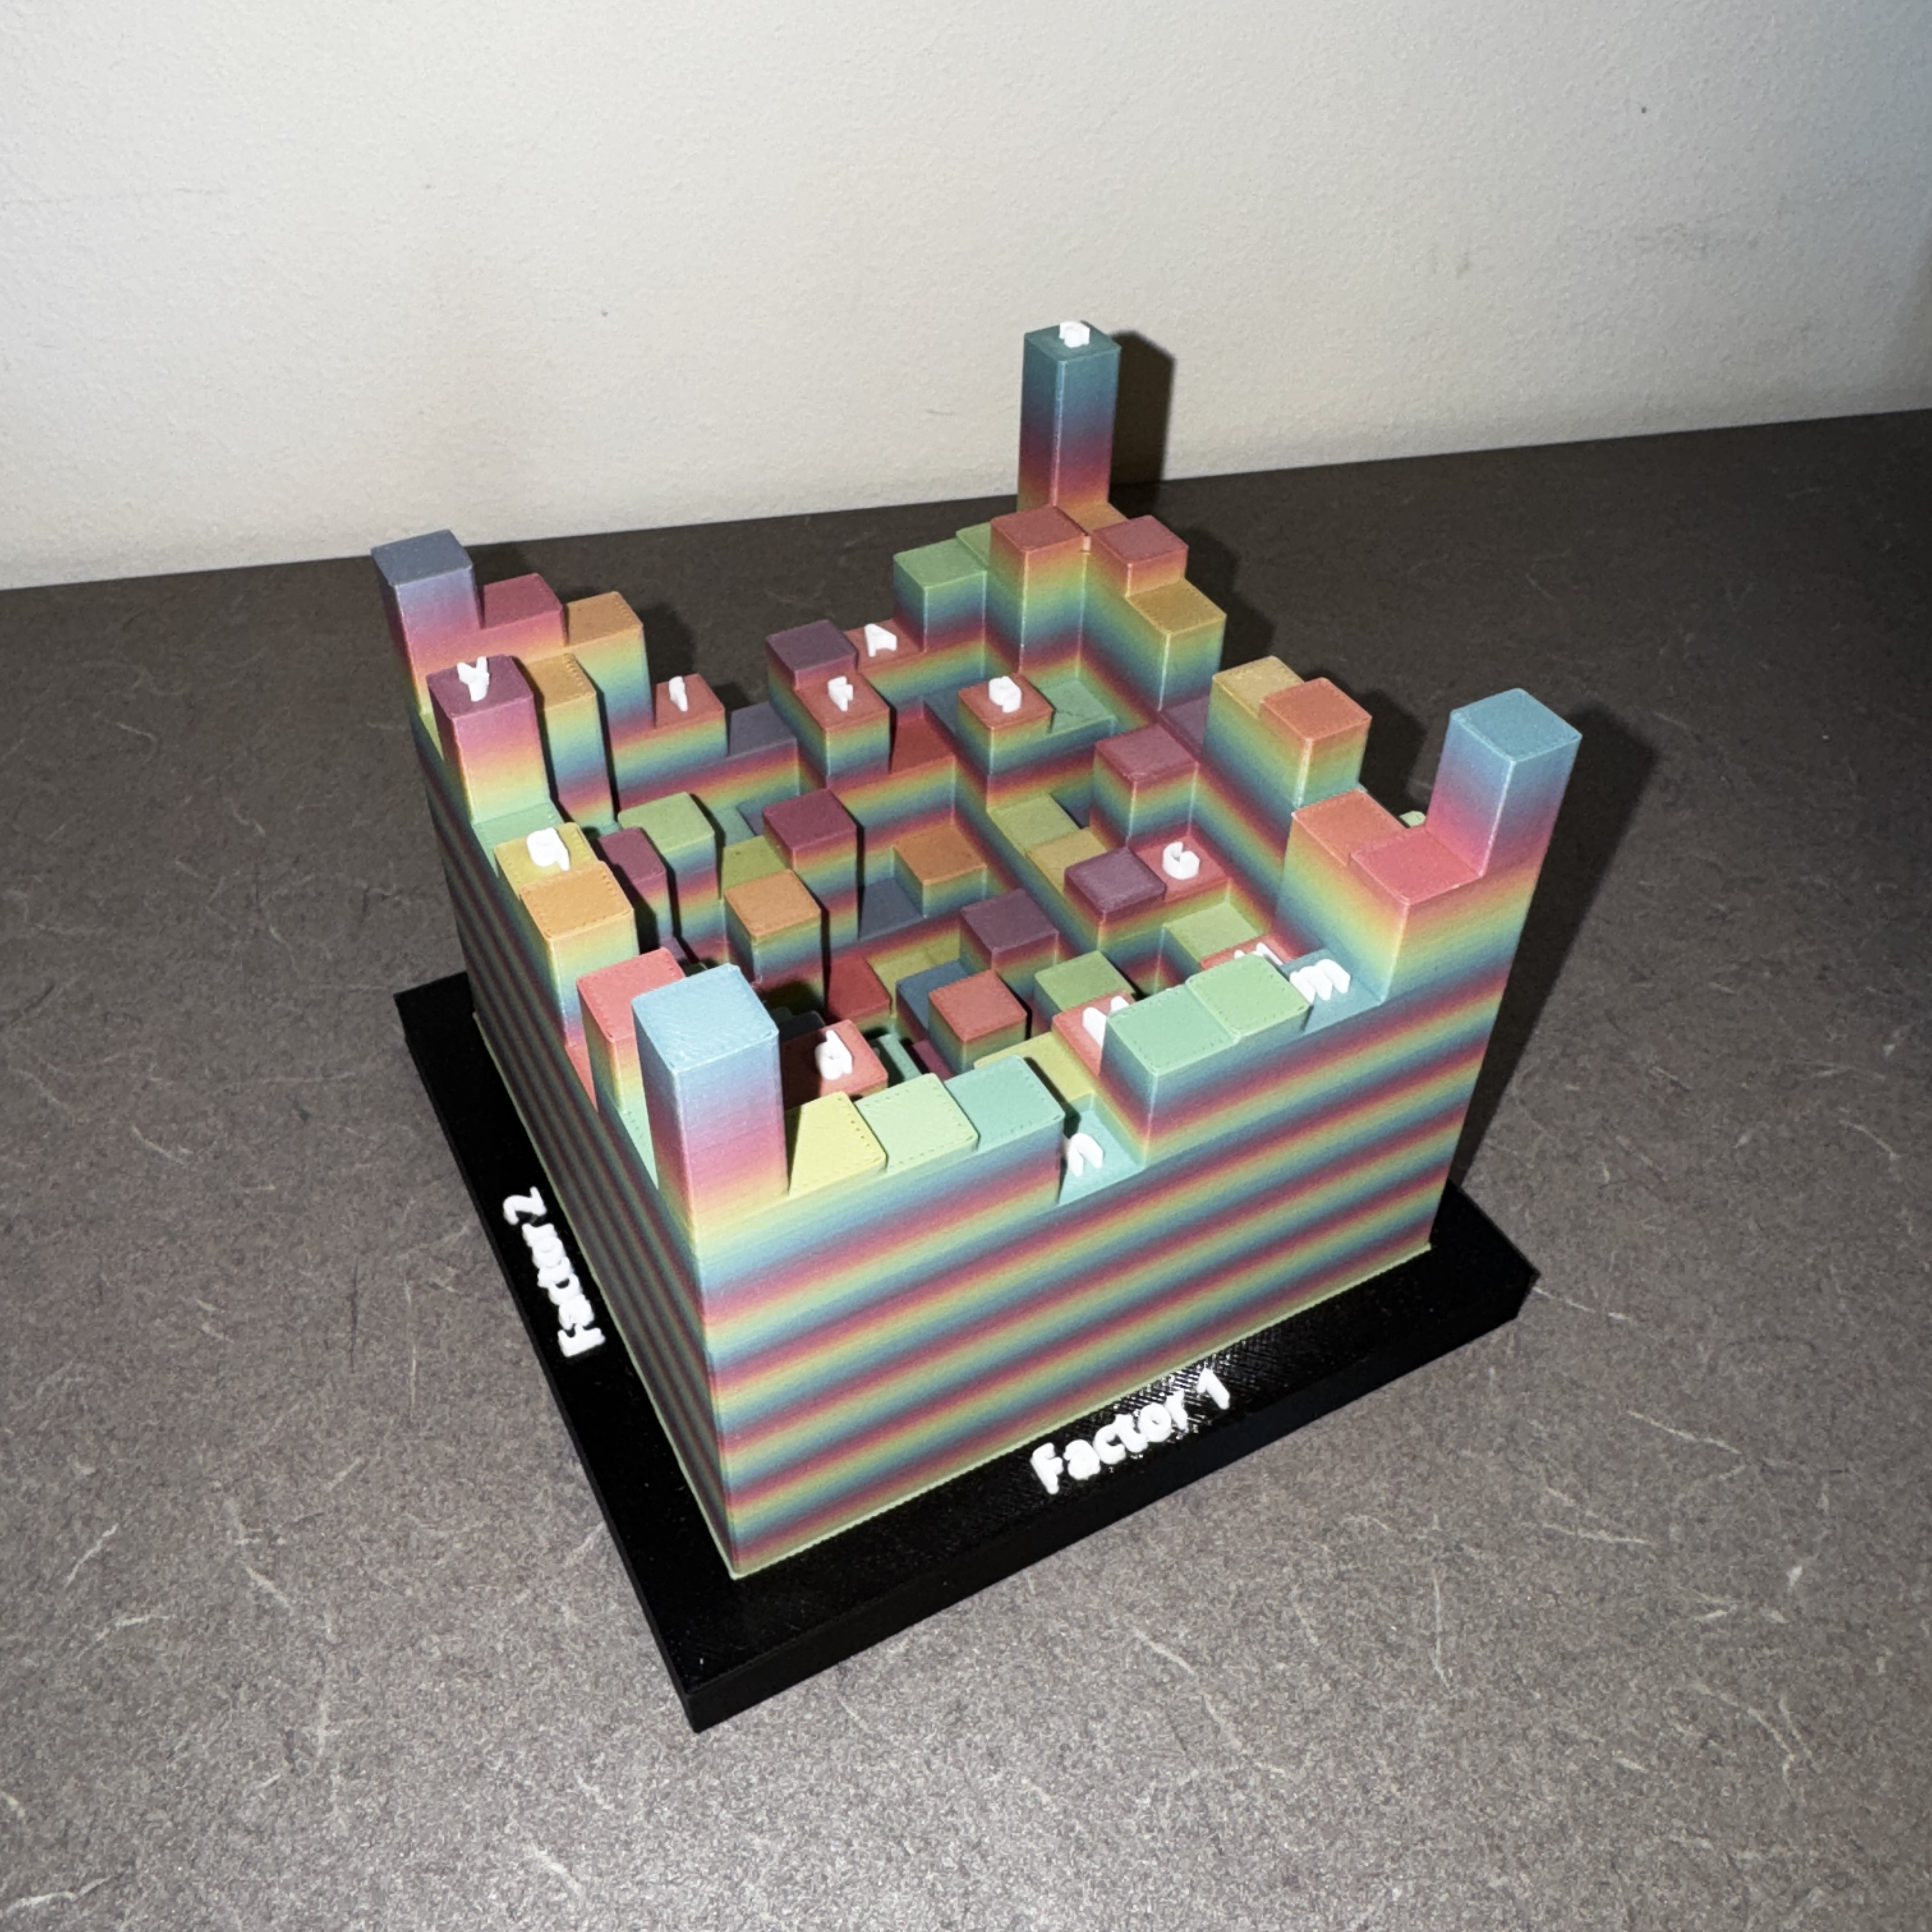
\includegraphics{images/3dp-gradient-set2.JPG}

}

\subcaption{\label{fig-3dp-solid}Data Set 2}

\end{minipage}%

\caption{\label{fig-3dp}3D printed heatmaps.}

\end{figure}%

To closely match the 3D-digital chart to the 3D-printed chart, multiple
stl files were created for each colored component and combined with the
RGL package (Murdoch and Adler 2023). The base was rendered with white
smoke (\#F5F5F5) to slightly contrast with the default white background
color (\#FFFFFF). Heatmap tiles were rendered with cyan (\#74CCFF) and
text labels were rendered with black (\#000000). Lighting was fixed at
45 degree angles at two opposite corners of the chart. The end result
was a near-perfect replica of the 3D-printed charts, with the exception
of different heatmap tile colors Figure~\ref{fig-3dd}.

\begin{figure}

\centering{

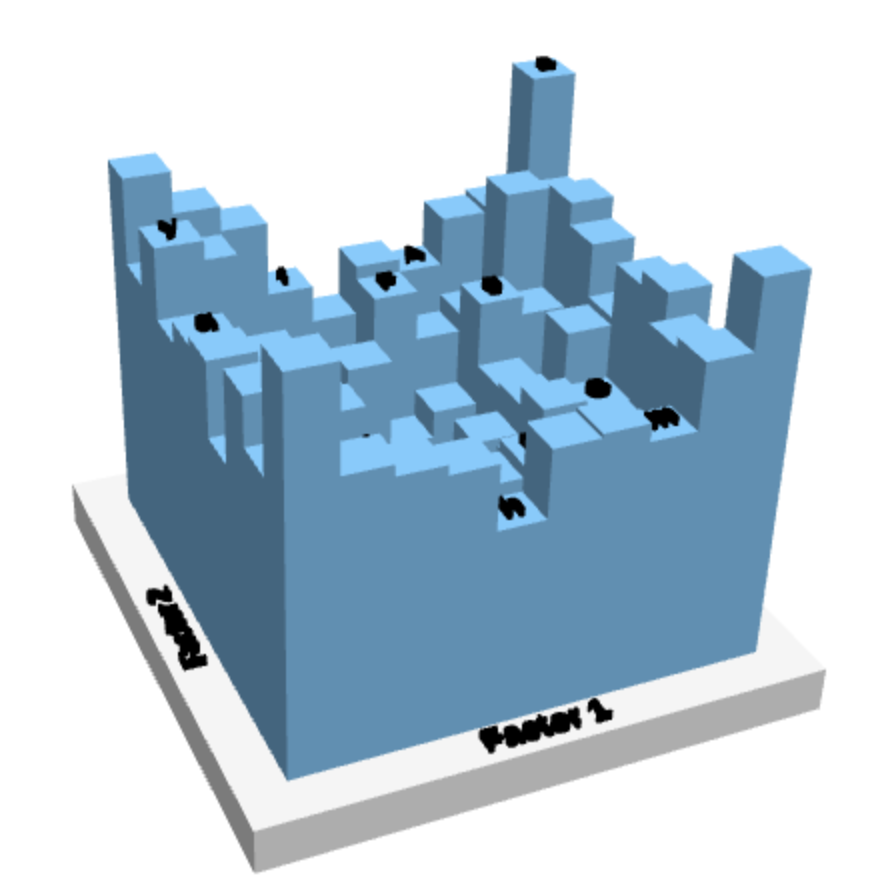
\includegraphics{images/chart-3dd.png}

}

\caption{\label{fig-3dd}RGL rendering of Data Set 2 for 3dd charts.}

\end{figure}%

Unlike the 3D charts, the 2D charts needed a different encoding to
convey heatmap values. The 2D heatmaps were created with
\texttt{ggplot2} (Wickham 2016) using \texttt{geom\_tile()}. Fill colors
for the cells use a color gradient ranging from Blue Zodiac (\#0C2841)
to Malibu (\#66D9FF), which were selected from a color picker using
shadows on our initial 3D-printed charts. The color interpolation was
performed with the \texttt{scale\_fill\_gradient()} function from the
\texttt{ggplot2} package.

\begin{figure}

\centering{


\includegraphics{index_files/figure-pdf/fig-color-pal-1.pdf}

}

\caption{\label{fig-color-pal}Color palette for 2D-digital charts. The
colors are interpolated from \#0C2841 to \#66D9FF, which are the colors
of the lighting conditions for a 3D-printed chart created with cyan
filament.}

\end{figure}%

\subsubsection{Subject Recruitment}\label{subject-recruitment}

Participants were recruited from STAT 218: \emph{Introduction to
Statistics} at the University of Nebraska-Lincoln in the summer and fall
of 2025. The experiment was incorporated into the curriculum as a
project that allowed students to get hands-on experience with
statistics. For data to be collected as part of our study, students had
to be at least 19 years old (age of majority in Nebraska) and consent to
participation.

STAT 218 is a general education statistics course at the University of
Nebraska. As such, many students enrolled in the course are in the 18-25
age range and are in the process of obtaining a Bachelor's degree. This
allowed for the unique opportunity for us to obtain a sample size that
is larger than typical studies in graphical perception, and that could
accommodate in-person participation required for the 3D printed charts.
Some sections of STAT 218 were held online in an asynchronous format.

\subsubsection{Experimental Design}\label{experimental-design}

Our experiment was designed with a 3 media type x 2 datasest x 9
comparison treatment structure. Media type is our main interest, with
2D-digital, 3D-digital, and 3D-printed charts. To ensure that results
are not confounded with datasets, we used two datasets, with a total of
9 stimuli pairs in each dataset. The order of treatments was given so
that media and dataset combinations were grouped together randomly in
the sequence with stimuli pairs randomized within the groupings. This
meant participants did not have to switch charts as frequently, reducing
the risk of using the wrong chart. For students enrolled in online
sections of STAT 218, the 3D-printed charts were removed from their
trials as they were not required to be on campus.

Due to practical constraints, stimuli pairs were incompletely blocked. A
full factorial design would result in 54 trials per participant, which
could lead to a decrease in quality responses (Herzog and Bachman 1981).
Therefore, we selected four out of the nine possible stimuli pairs to
create incomplete blocks for each chart. This resulted in 18 blocks for
a balanced incomplete block design. Within each block, media type is
fully crossed with dataset. Using the incomplete block structure,
participants completed a total of 24 trials, which is more practical
than the full factorial design.

Following the procedure of Cleveland and McGill (1984), we asked
participants two questions in each trial. The first question asked
participants which stimuli in a specified pair is larger or if the
stimuli are the same value. Next, participants were asked to estimate
the magnitude of the smaller stimuli if the larger stimuli represents
100 units, which is a subtractive process (Veit 1978). This question is
designed to estimate \(A/B\), where \(A\leq B\).

\paragraph{Shiny Application}\label{shiny-application}

A Shiny application (Chang et al. 2024) was developed to administer the
experiment. The application consisted of five sections: informed
consent, demographics, practice, experiment, and wrap-up. The entire
application was designed to be completed in approximately 30 minutes.

The Shiny application started with the informed consent screen, allowing
participants to select if they are a STAT 218 Student and if they agree
to the data collection. Participants had to select a data collection
option to continue. After submitting their data collection response, a
completion code was generated and saved on the last page of the
application. This code was required for class, but participant consent
was only required to save the data, so underage participants could still
get the code for course credit.

If participants agreed to have their data collected, they were presented
with the demographics section. This section asked participants about
their age, gender identity, highest education level, and how their
participation in the experiment is graded. The last question was a text
box and asked participants to specify their favorite movie and/or actor.
Demographic information was combined with the application start time and
completion code to create a hash for an anonymized participant
identifier using the \texttt{rlang} package (Henry and Wickham 2025).

Once a participant completed the demographics page or selected ``No'' to
the data collection question, they were given a practice page. A modal
dialog window was initially shown with instructions, and users could
display this window again at any point during the practice trials. The
practice consisted of four questions: two trials from 2dd charts and two
trials from 3dd charts. Once participants provided a response to both
questions in a practice trial, they were able to display the correct
solution to check their answers. Since the practice trials were only to
inform participants about the mechanics for answering the questions, we
did not include 3D-printed charts. This eliminated the possibility of
participants using a practice chart for the experiment.

The experiment page was presented to participants after completion of
the practice trials Figure~\ref{fig-exp-page}. Each page contained two
questions -- one question for identifying which stimuli is larger and
another question for estimating the value of the smaller stimuli if the
larger stimuli is 100 units. Each trial had the initial slider position
randomized in order to prevent starting position bias. For 3dd charts,
the number of interactive clicks was also recorded. A trial could only
be submitted if the first question is answered and if the slider was
moved at least once.

\begin{figure}

\centering{

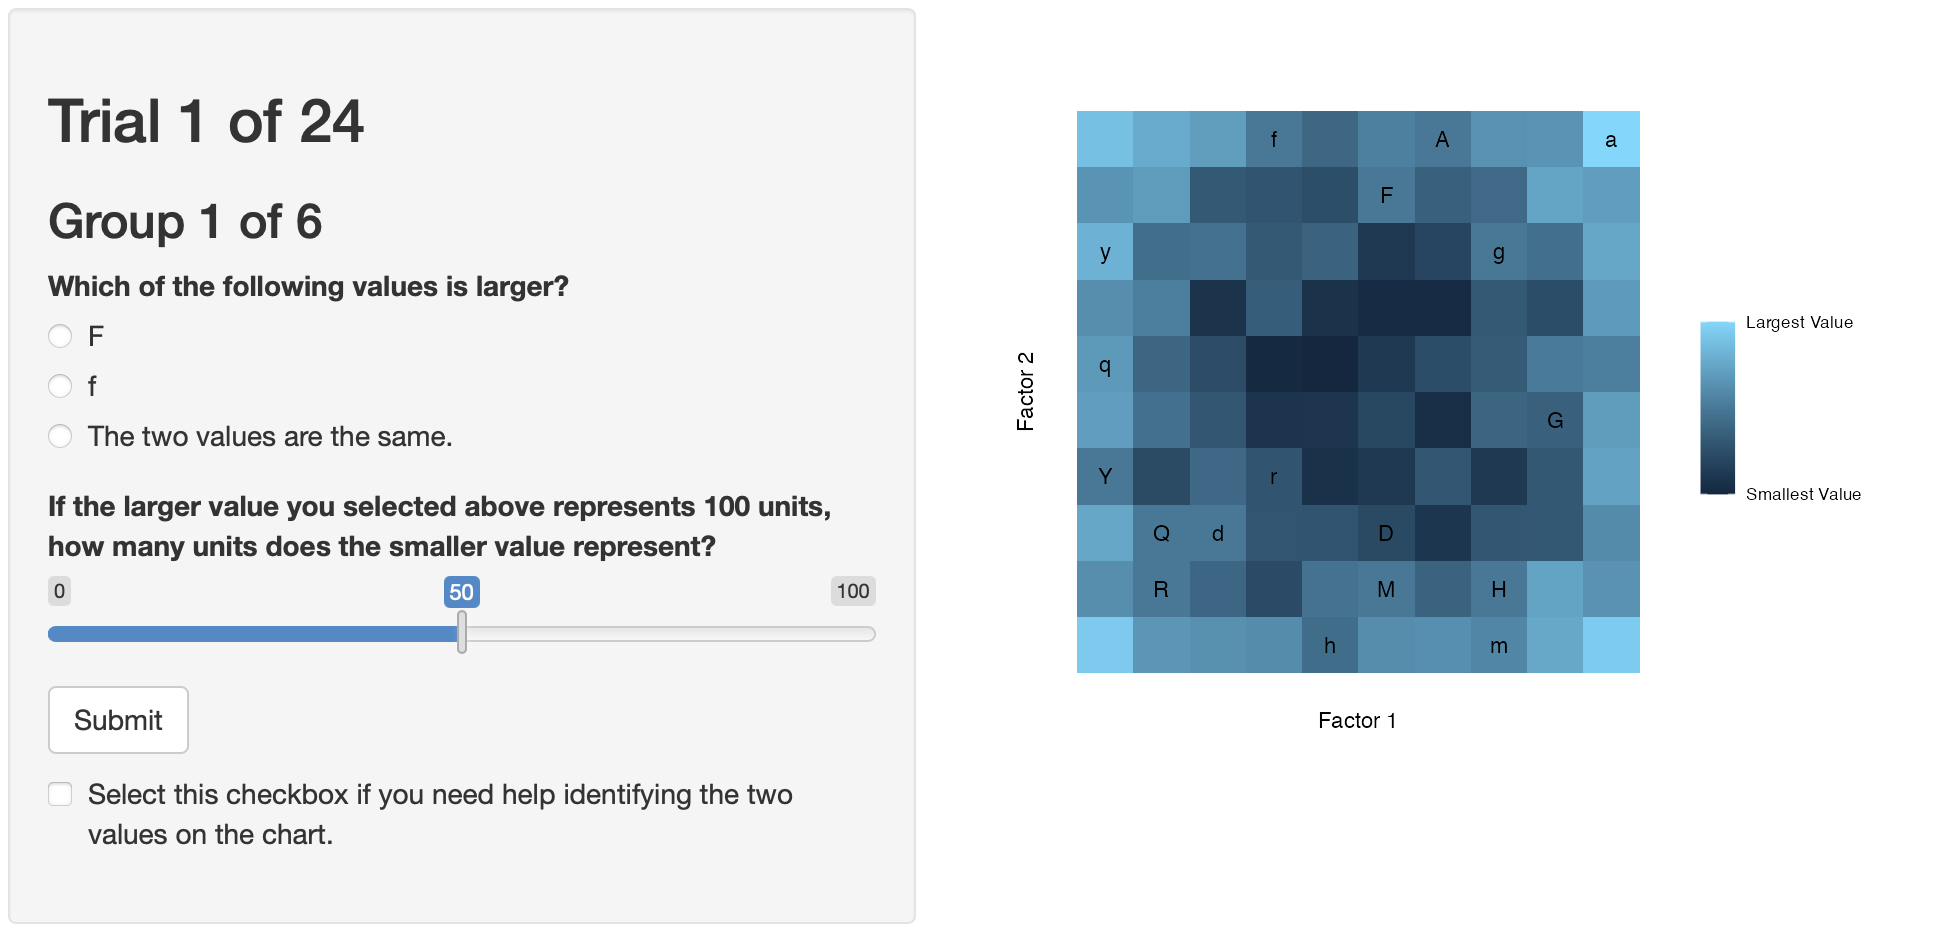
\includegraphics[width=1\textwidth,height=\textheight]{images/experiment-page.png}

}

\caption{\label{fig-exp-page}Graphics experiment page. Each trial
contained two questions about a pair of stimuli, and a check box that
displays the location of the stimuli if needed.}

\end{figure}%

After completing all trials, participants were given the completion code
and informed to provide the code to their instructor since they would
not have access to the code after closing out of the experiment.

\paragraph{Method of Analysis}\label{method-of-analysis}

The design of our experiment is a balanced incomplete split-plot with
replication, where media type and dataset are whole-plot factors for
each participant and stimuli pair is the split plot. A similar design
was presented by Mandal, Parsad, and Dash (2020) for a single replicate.
For our analysis, we used the following model as a baseline:

\[
Y_{ijklm}=\mu+S_i\times M_j\times P_k+\gamma_{lm}+\omega_{ijlm}+\epsilon_{ijklm}
\]

In our model, \(Y_{ijklm}\) is a metric of error for participant
responses to the ratio estimation question, \(S_i\) is the effect of
dataset \(i\), \(M_j\) is the effect of chart type \(j\), \(P_k\) is the
effect of stimuli pair \(k\), and \(S_i\times M_j\times P_k\) includes
all corresponding main effects and two-way and three-way interactions.
Our random effects include \(\gamma_{lm}\sim N(0,\sigma^2_A)\) for
participant \(m\) in block \(l\), \(\omega_{ijlm}\sim N(0,\sigma^2_B)\)
for the ordering of dataset \(i\) and chart type \(j\) for participant
\(m\) in block \(l\), and \(\epsilon_{ijklm}\sim N(0, \sigma^2_C)\) for
the residual error. We assume that \(\gamma_{lm}\), \(\omega_{ijlm}\),
and \(\epsilon_{ijklm}\) are independently and identically distributed.

The first question in each trial was to indicate which value within a
stimulus pair was larger, or if they were the same value. Following
Cleveland and McGill (1984), we use this question as an attention check
to verify that participants are following the procedure and that the
correct comparison is being made.

\subsection{Results}\label{results}

In this section, we describe the demographic information of our sample,
cleaning of participant responses, analysis of responses, and
interactions participants had with the Shiny application.

\subsubsection{Demographics}\label{demographics}

Our experiment was conducted with eight sections of Stat 218 between
August 25th and December 19th in 2025 at the University of Nebraska. To
participate in the experiment, students were instructed to visit
communal office hour locations to access the 3D printed charts. We
recorded 482 interactions with the shiny application, of which 259
students completed the entirety of the experiment. Of these students, 92
were enrolled in online sections of the course and did not have access
to the 3D printed charts. The vast majority of participants were
actively completing their undergraduate degree and between the ages of
19 and 25. Full demographic information can be found in
Table~\ref{tbl-demographics}.

\begin{table}

\caption{\label{tbl-demographics}Demographic Information}

\centering{

\centering
\begin{tabular}[t]{lrr}
\toprule
 & Count & Proportion\\
\midrule
\addlinespace[0.3em]
\multicolumn{3}{l}{\textbf{Gender}}\\
\hspace{1em}Female & 166 & 0.64\\
\hspace{1em}Male & 90 & 0.35\\
\hspace{1em}Variant/Nonconforming & 1 & 0.00\\
\hspace{1em}Prefer not to answer & 2 & 0.01\\
\addlinespace[0.3em]
\multicolumn{3}{l}{\textbf{Age}}\\
\hspace{1em}19-25 & 252 & 0.97\\
\hspace{1em}26-30 & 2 & 0.01\\
\hspace{1em}31-35 & 0 & 0.00\\
\hspace{1em}36-40 & 1 & 0.00\\
\hspace{1em}41-45 & 3 & 0.01\\
\hspace{1em}Prefer not to answer & 1 & 0.00\\
\addlinespace[0.3em]
\multicolumn{3}{l}{\textbf{Education}}\\
\hspace{1em}High School or Less & 23 & 0.09\\
\hspace{1em}Some Undergraduate Courses & 214 & 0.83\\
\hspace{1em}Undergraduate Degree & 12 & 0.05\\
\hspace{1em}Some Graduate Courses & 4 & 0.02\\
\hspace{1em}Graduate Degree & 2 & 0.01\\
\hspace{1em}Prefer not to answer & 4 & 0.02\\
\bottomrule
\end{tabular}

}

\end{table}%

Almost all participants completed the experiment in under 20 minutes.
Summary statistics can be found in Table~\ref{tbl-exp-times}, with the
overall distribution of times shown in Figure~\ref{fig-total-time}.
Individual trials had a median completion time of 0.23 minutes.

\begin{longtable}[]{@{}lrrr@{}}

\caption{\label{tbl-exp-times}Summary of experiment completion times in
minutes.}

\tabularnewline

\toprule\noalign{}
Section & Mean & SD & Median \\
\midrule\noalign{}
\endhead
\bottomrule\noalign{}
\endlastfoot
In-person & 8.08 & 3.39 & 7.45 \\
Online & 5.70 & 3.42 & 5.09 \\
All Participants & 7.23 & 3.58 & 6.86 \\

\end{longtable}

\begin{figure}

\centering{

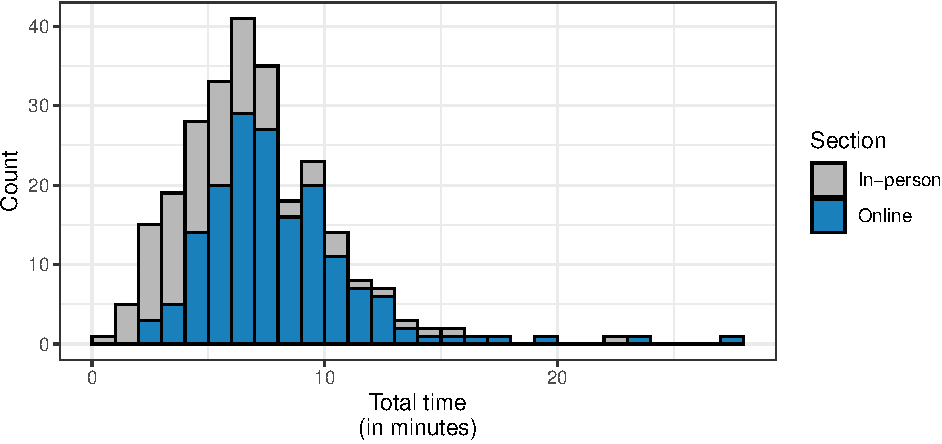
\includegraphics{index_files/figure-pdf/fig-total-time-1.pdf}

}

\caption{\label{fig-total-time}Histogram of experiment completion times.
Online participants had generally shorter completion times due to a
decreased number of trials.}

\end{figure}%

During our initial exploration of the results, we discovered a
non-negligible number of students who did not follow the instructions,
which is not surprising in an intro statistics class activity. In some
cases, participants appeared to be using alternative estimation
strategies, such as estimating the difference between the two values in
a stimulus pair, rather than the specified ratio strategy. Additionally,
we noticed that several students were randomly entering values in order
to obtain the completion code at the end of the experiment. We provide
some examples of individual participant responses in
Figure~\ref{fig-user-strategies} to illustrate this issue.

\begin{figure}

\centering{

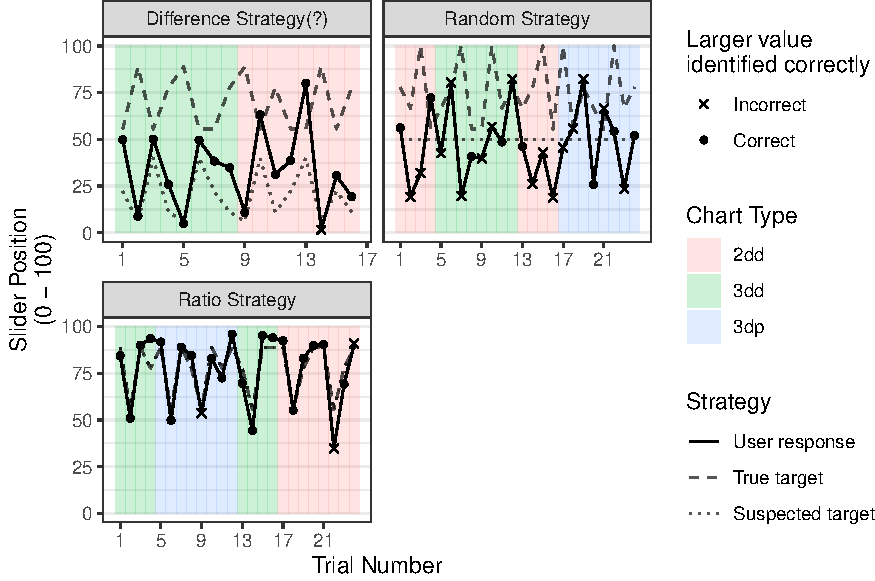
\includegraphics{index_files/figure-pdf/fig-user-strategies-1.pdf}

}

\caption{\label{fig-user-strategies}Three potential estimation
strategies from participants. Many participants followed instructions to
estimate ratios. However, some participants appeared to estimate the
difference between stimuli pairs or submitted random values.}

\end{figure}%

It is commonly acknowledged in psychology that careless respondents
should be addressed to some degree, although there is no general
consensus on how to handle this without cherry picking (Jaso, Kraus, and
Heller 2021; Ward and Meade 2023). Some proposed solutions include
removing participants based on observed patterns or fitting mixture
models to address latent class variables. In this section, we discuss
one possible subset of participant responses to address careless
respondents. We also include several alternative models in the appendix.

\subsubsection{Addressing Random Categorical
Responses}\label{sec-remove-random-categories}

To improve the quality of our data, we started by assessing random
guesses in identifying the larger value of a stimulus pair. In each
trial, participants have a 1 out of 3 chance for correctly identifying
the larger value if they are randomly guessing. Since stimuli pair 5
contains identical values, we temporarily exclude those trials to focus
on stimuli pairs where there was a difference between the values. For
each participant, we test \(H_0: \pi\leq2/3\text{ vs. }H_1:\pi>2/3\)
with \(\alpha=0.05\), where \(\pi\) is the probability of a participant
correctly answering the initial question and \(\alpha\) is the level of
the test. That is, participants who are following instructions should
select the correct option at least twice as often as either incorrect
alternative. Given the lack of standardized criteria for identifying
careless responding, the one-sided Binomial test should extract users
who are suspected to be following the instructions. Using the first
question for participant screening, 98 participants are excluded for
suspected random selecting, leaving 161 participants. The effect of this
exclusion can be seen in Figure~\ref{fig-q1-eda}.

\begin{figure}

\begin{minipage}{0.50\linewidth}

\centering{

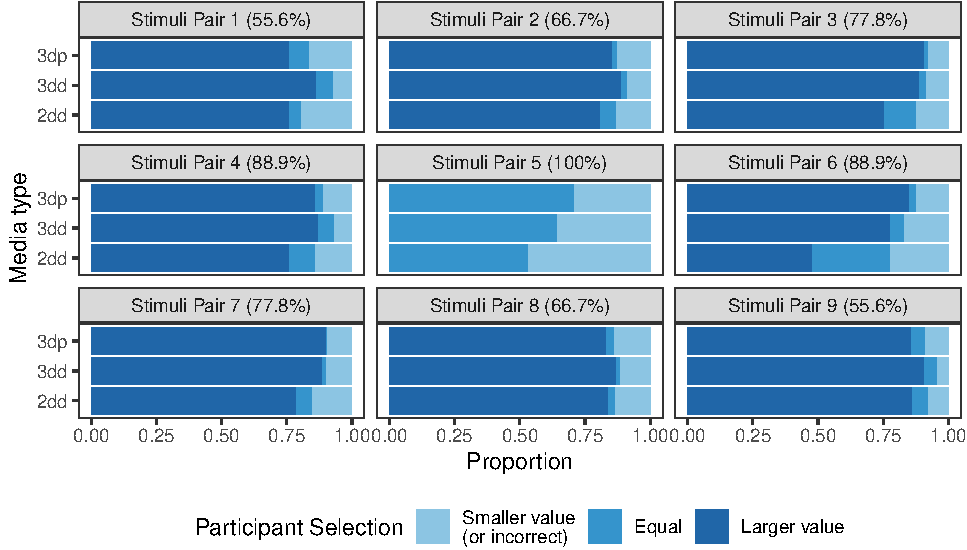
\includegraphics[width=0.9\textwidth,height=\textheight]{index_files/figure-pdf/fig-q1-eda-1.pdf}

}

\subcaption{\label{fig-q1-eda-1}No participant filtering}

\end{minipage}%
%
\begin{minipage}{0.50\linewidth}

\centering{

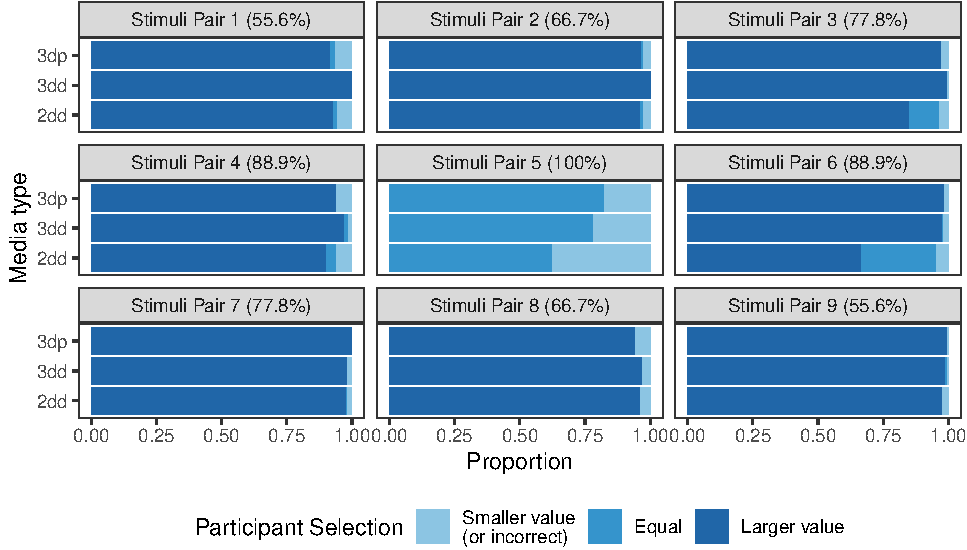
\includegraphics[width=0.9\textwidth,height=\textheight]{index_files/figure-pdf/fig-q1-eda-2.pdf}

}

\subcaption{\label{fig-q1-eda-2}Exclude random guessers}

\end{minipage}%

\caption{\label{fig-q1-eda}Proportion of correct responses to Question 1
across stimuli pairs and media types. For all pairs, with the exception
of Pair 5, a correct answer was `Larger value'. Stimuli Pair 5 had two
identical values, meaning that options other than `Both values are the
same' were incorrect.}

\end{figure}%

\subsubsection{Analysis of Error}\label{analysis-of-error}

We follow the same calculation of error as Cleveland and McGill (1984),
which is shown in Equation~\ref{eq-error_cm}. Error is defined as the
base-2 logarithm of the absolute estimation error meaning that
differences of one unit on this scale correspond to approximately
doubling the size of the error. The addition of 1/8 prevents distortion
for responses with near-zero error.

\begin{equation}\phantomsection\label{eq-error_cm}{
y=\log_2(|\text{User Response}-100\times(\text{True ratio})|+1/8)
}\end{equation}

In our analysis, we excluded individual responses where participants
were incorrect in their response to the initial question and all
responses for stimuli pair 5. The initial question served as an
attention check to verify that the participants were making the correct
comparison between stimuli values. For stimuli pair 5, we removed these
trials since correct solutions should be a binary response. However, we
discovered a discrepancy in how participants were responding to both
questions for these trials, which we discuss in the appendix.

With our specified exclusion criteria, we find that there was marginal
evidence for the effects of chart type (p-value = 0.041) and the data
set and stimuli pair interaction (p-value = 0.073). This finding is
consistent with models fitted with various participant and response
filters.

Our findings suggest that the 2D heatmaps had evidence of higher log
absolute error than either type of the 3D heatmaps. On the base-2 log
scale, the error for 2D heatmaps was larger than the error for digital
3D heatmap by 0.414 (95\% CI: 0.253, 0.574). This finding is similar for
the 3D printed heatmaps, where the log absolute error for 2D heatmaps
was larger by 0.413 (95\% CI: 0.234, 0.591). There were no detectable
differences in error between the digital and physical 3D heatmaps
(p-value = 1).

\begin{figure}

\centering{

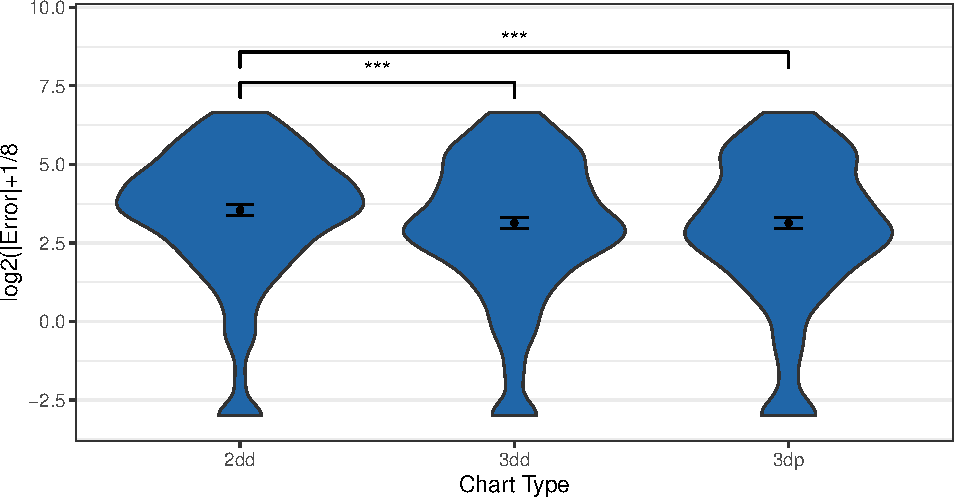
\includegraphics{index_files/figure-pdf/fig-em-media-1.pdf}

}

\caption{\label{fig-em-media}Distributions of log error overlayed with
estimated marginal means and their 95\% confidence intervals.
Differences were only detected between 2D heatmap and both types of 3D
heatmaps, where the 2D heatmap had evidence of larger errors.}

\end{figure}%

When examining the interaction between stimuli pairs and underlying
datasets, 11 differences in log absolute error were detected at the
\(\alpha=0.05\) level. Seven of these differences occurred with stimuli
pair 6 (ratio = 0.889) and dataset 1, which had the smallest estimated
marginal mean of log absolute error. All differences can be found in
Figure~\ref{fig-em-set-pair}, where significant differences are assessed
via a compact letter display from the \texttt{multcomp} package
(Hothorn, Bretz, and Westfall 2008).

\begin{figure}

\centering{

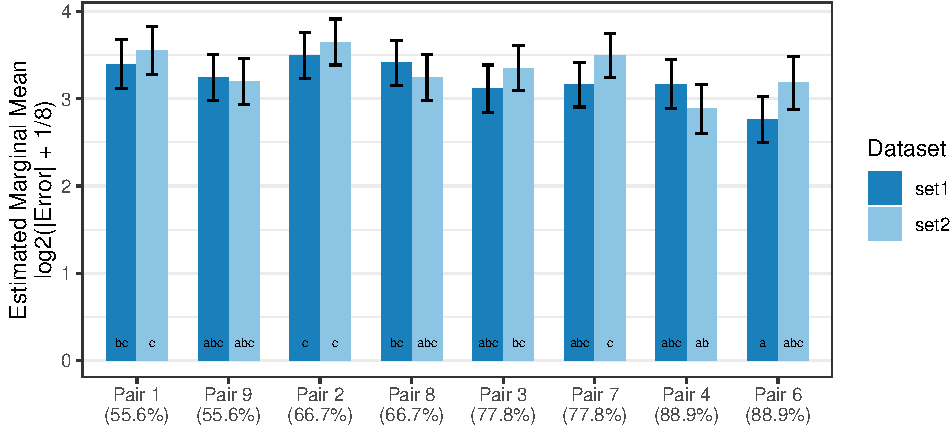
\includegraphics{index_files/figure-pdf/fig-em-set-pair-1.pdf}

}

\caption{\label{fig-em-set-pair}Estimated marginal means of stimuli pair
and dataset. Bars sharing the same letter are not significantly
different from one another.}

\end{figure}%

\subsubsection{Participant Interactions with Shiny
Application}\label{participant-interactions-with-shiny-application}

In this section, we describe participant interactions with the Shiny
application using the same participant exclusion criteria as our model.
As participants completed the experiment, we recorded the amount of time
to complete each trial, the number of cursor clicks on the digital 3D
heatmaps, and the number of times that the slider was moved. We also
recorded the initial starting position of the slider, which was randomly
placed for each trial.

Many participants completed each trial in under 20 seconds. The median
completion time was 14.8372396 seconds, with a standard deviation of
22.9971286 seconds. There were 91 participants who had at least one
trial exceed 60 seconds. Due to the design and administration of the
experiment, we are unable to account for the cause of longer trial
completion times, but it is possible the students may have been
interrupted or distracted before returning to the task.

\begin{figure}

\begin{minipage}{0.50\linewidth}

\centering{

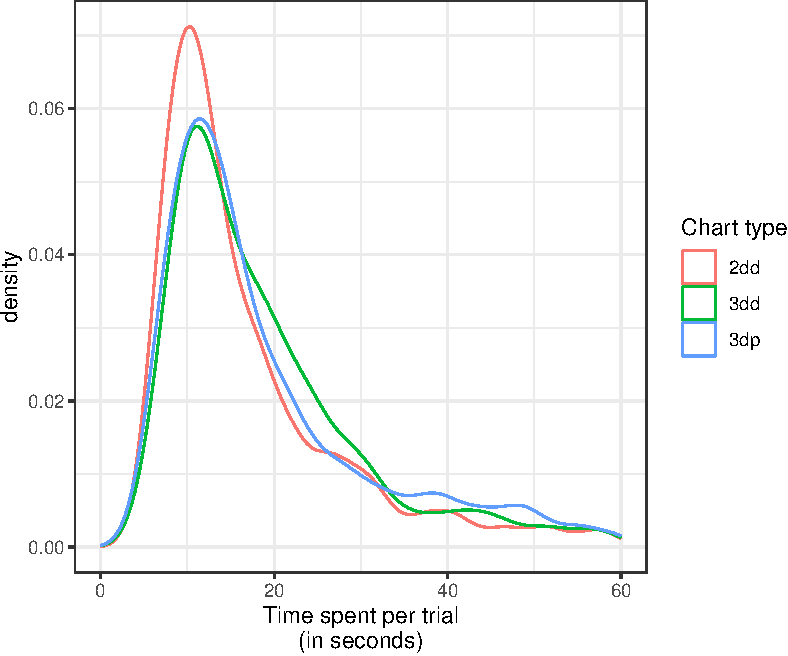
\includegraphics[width=0.9\textwidth,height=\textheight]{index_files/figure-pdf/fig-time-summary-1.pdf}

}

\subcaption{\label{fig-time-summary-1}Frequency plot}

\end{minipage}%
%
\begin{minipage}{0.50\linewidth}

\centering{

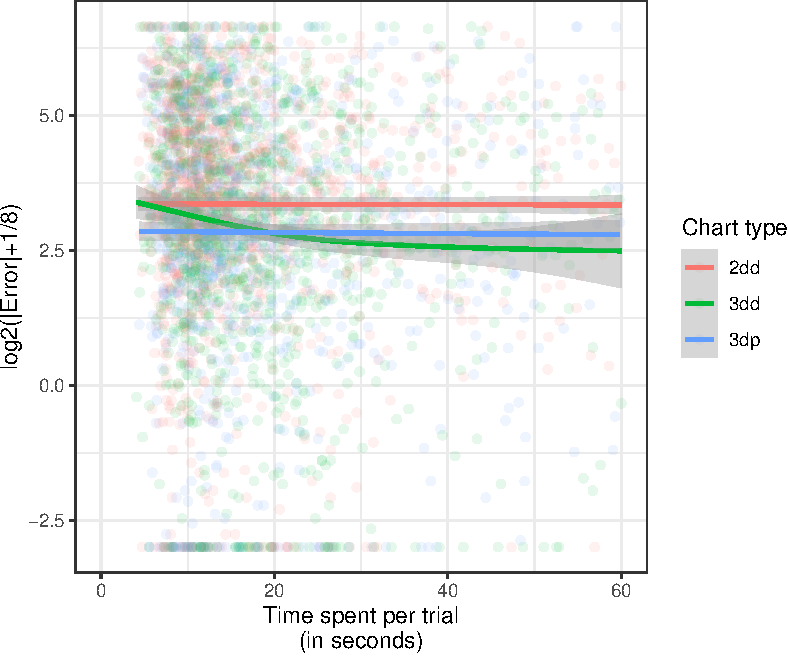
\includegraphics[width=0.9\textwidth,height=\textheight]{index_files/figure-pdf/fig-time-summary-2.pdf}

}

\subcaption{\label{fig-time-summary-2}Time vs.~Error}

\end{minipage}%

\caption{\label{fig-time-summary}Visual summary of time spent on each
trial. 137 trials are omitted due to lasting longer than 60 seconds.}

\end{figure}%

\begin{figure}

\begin{minipage}{0.50\linewidth}

\centering{

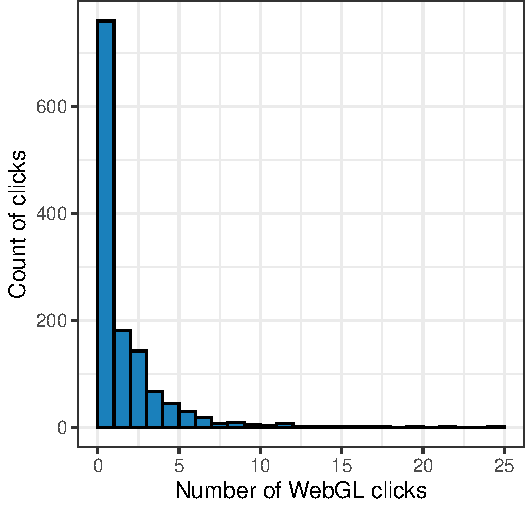
\includegraphics[width=0.9\textwidth,height=\textheight]{index_files/figure-pdf/fig-clicks3dd-1.pdf}

}

\subcaption{\label{fig-clicks3dd-1}Histogram}

\end{minipage}%
%
\begin{minipage}{0.50\linewidth}

\centering{

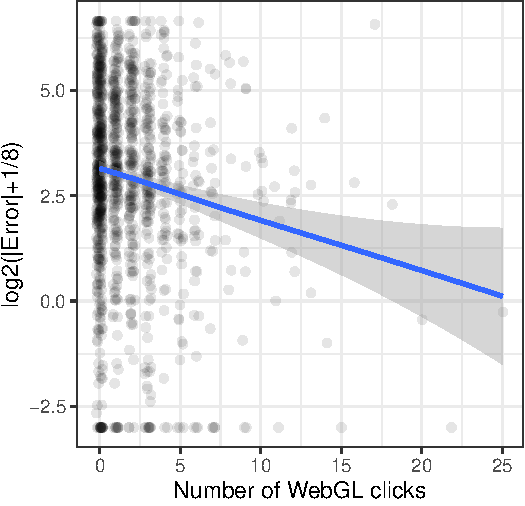
\includegraphics[width=0.9\textwidth,height=\textheight]{index_files/figure-pdf/fig-clicks3dd-2.pdf}

}

\subcaption{\label{fig-clicks3dd-2}WebGL clicks vs.~Error}

\end{minipage}%

\caption{\label{fig-clicks3dd}Participant interactions with the digital
3D heatmaps.}

\end{figure}%

\begin{figure}

\begin{minipage}{0.50\linewidth}

\centering{

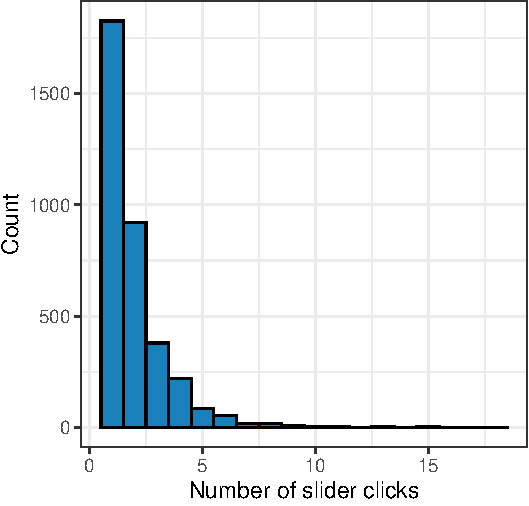
\includegraphics[width=0.9\textwidth,height=\textheight]{index_files/figure-pdf/fig-slider-clicks-1.pdf}

}

\subcaption{\label{fig-slider-clicks-1}Histogram}

\end{minipage}%
%
\begin{minipage}{0.50\linewidth}

\centering{

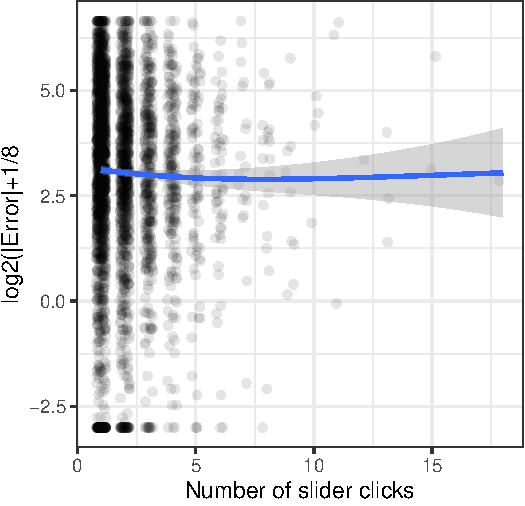
\includegraphics[width=0.9\textwidth,height=\textheight]{index_files/figure-pdf/fig-slider-clicks-2.pdf}

}

\subcaption{\label{fig-slider-clicks-2}Slider clicks vs.~Error}

\end{minipage}%

\caption{\label{fig-slider-clicks}Participant interactions with the
slider.}

\end{figure}%

\begin{figure}

\centering{

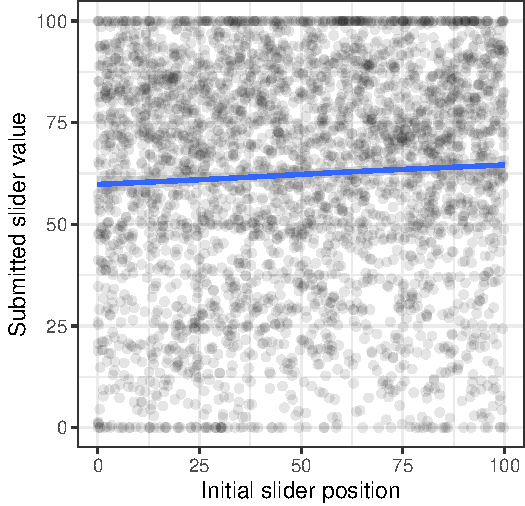
\includegraphics{index_files/figure-pdf/fig-slider-start-1.pdf}

}

\caption{\label{fig-slider-start}Effect of initial slider position on
the submitted slider value.}

\end{figure}%

\subsection{Discussion and Conclusion}\label{discussion-and-conclusion}

Our study was designed to test the numerical estimation of ratios in 2D
and 3D heatmaps rendered in digital and physical environments. The
current state of tangible statistical graphics is limited mainly to
tactile displays, whereas 3D printed statistical graphics are largely
unexplored. We found that when the third dimension is conveying
meaningful information, the heights of 3D heatmaps had smaller errors
than the color gradient of 2D heatmaps. No differences were detected
between the digital and physical 3D heatmaps, which is perhaps
attributed to the exact one-to-one design relationship between the
digital display and the 3D printed chart. These findings were consistent
across multiple levels of fitted models and participant filtering, which
reaffirms our belief that 3D charts have value when meaningfully using
all three dimensions.

An interesting observation from the stimuli pairs and dataset
interaction was from the non-detectable differences. We note that no
differences were detected across datasets for a given stimuli pair.
While not explicitly tested in our experiment, there have been previous
studies that have investigated and found the behavior of neighboring
values to have an effect (Zacks et al. 1998; VanderPlas and Hofmann
2015). This effect would be worth exploring in future studies with 3D
heatmaps. Another concern we had when designing our experiment was the
lack of direct translation from color scales to heights. The differences
between stimuli pairs of identical ratios were non-detectable, which
alleviates this concern for future studies. However, this effect would
likely be important to consider if assessing just noticeable differences
(Lu et al. 2022; Zhang et al. 2023).

While our hypothesis that 3D-printed heatmaps would outperform digital
2D and 3D heatmaps in numerical estimations of ratios was not supported,
we were able to show that 3D charts may have a place in the analysis of
data. When the third dimension is used to display information, the
mapping of that dimension to height provides better ratio estimations
than a color gradient scale. This result has been observed previously in
digital 3D heatmaps (Barfield and Robless 1989; Kraus et al. 2020), and
our findings suggests that this may hold for physical 3D heatmaps.

\subsection{Appendix}\label{appendix}

In this section, we include multiple models for the transparency of
model selection. Visual inspections of participant responses indicate
that several participants clearly did not follow instructions by either
using alternate estimation strategies or by carelessly responding
Figure~\ref{fig-q1-eda}. While we should take these cases into
consideration, there is no singular solution to suggest a ``best'' model
(Jaso, Kraus, and Heller 2021; Ward and Meade 2023). Our purpose for
including these alternate models is to examine model sensitivity to
results through various levels of participant and response filtering.

For each model, we exclude stimuli pair 5. In theory, participants who
answer this question correctly will select that both values are the same
and move the slider to 100. From the included participants, as described
in Section~\ref{sec-remove-random-categories}, virtually all
participants who put the slider at 100 answered the first question
correctly. However, nearly 60 percent of responses indicated that the
values were the same in the first question but did not move the slider
to 100. Several factors could have attributed to this, such as slider
sensitivity or participants using alternate estimation strategies.
Rather than correcting what we think participants should have answered,
we removed this stimuli pair and motivate future research into ``just
noticeable differences'' for 3D heatmaps.

\begin{figure}

\centering{


\includegraphics{index_files/figure-pdf/fig-pair5-issues-1.pdf}

}

\caption{\label{fig-pair5-issues}Counts of response behavior for Stimuli
Pair 5. This pair had identical values, which means that true solutions
indicates marking that they were the same value and positioning the
slider at 100.}

\end{figure}%

There are multiple levels of participant and response filtering that we
considered. For participant-level filtering, we consider the following
levels: (1) no participant filtering and (2) remove suspected random
guessers. The process of (2) was described in
Section~\ref{sec-remove-random-categories}. Filtering individual
responses is a straightforward process, where we considered (i) include
all responses, and (ii) remove responses with incorrect Q1 solutions.

\begin{longtable}[]{@{}
  >{\raggedright\arraybackslash}p{(\columnwidth - 8\tabcolsep) * \real{0.1200}}
  >{\raggedleft\arraybackslash}p{(\columnwidth - 8\tabcolsep) * \real{0.2133}}
  >{\raggedleft\arraybackslash}p{(\columnwidth - 8\tabcolsep) * \real{0.1933}}
  >{\raggedleft\arraybackslash}p{(\columnwidth - 8\tabcolsep) * \real{0.2467}}
  >{\raggedleft\arraybackslash}p{(\columnwidth - 8\tabcolsep) * \real{0.2267}}@{}}
\caption{ANOVA Table p-values for model terms}\tabularnewline
\toprule\noalign{}
\begin{minipage}[b]{\linewidth}\raggedright
Term
\end{minipage} & \begin{minipage}[b]{\linewidth}\raggedleft
All participants, all responses
\end{minipage} & \begin{minipage}[b]{\linewidth}\raggedleft
All participants, Q1 correct
\end{minipage} & \begin{minipage}[b]{\linewidth}\raggedleft
Filtered participants, all responses
\end{minipage} & \begin{minipage}[b]{\linewidth}\raggedleft
Filtered participants, Q1 correct
\end{minipage} \\
\midrule\noalign{}
\endfirsthead
\toprule\noalign{}
\begin{minipage}[b]{\linewidth}\raggedright
Term
\end{minipage} & \begin{minipage}[b]{\linewidth}\raggedleft
All participants, all responses
\end{minipage} & \begin{minipage}[b]{\linewidth}\raggedleft
All participants, Q1 correct
\end{minipage} & \begin{minipage}[b]{\linewidth}\raggedleft
Filtered participants, all responses
\end{minipage} & \begin{minipage}[b]{\linewidth}\raggedleft
Filtered participants, Q1 correct
\end{minipage} \\
\midrule\noalign{}
\endhead
\bottomrule\noalign{}
\endlastfoot
set & 0.340 & 0.705 & 0.939 & 0.735 \\
media & 0.010 & 0.018 & 0.035 & 0.041 \\
pair\_id & 0.244 & 0.333 & 0.089 & 0.063 \\
set:media & 0.297 & 0.711 & 0.543 & 0.669 \\
set:pair\_id & 0.003 & 0.145 & 0.001 & 0.073 \\
media:pair\_id & 0.815 & 0.740 & 0.982 & 0.968 \\
set:media:pair\_id & 0.489 & 0.764 & 0.255 & 0.833 \\
\end{longtable}

\begin{figure}

\centering{

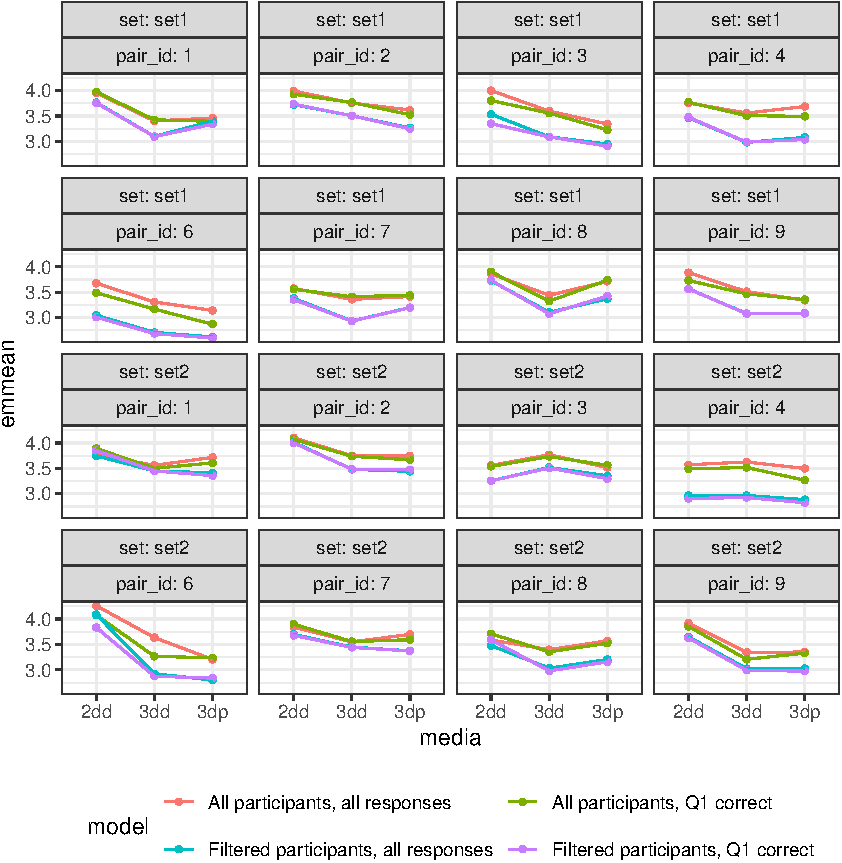
\includegraphics{index_files/figure-pdf/fig-model-int1-1.pdf}

}

\caption{\label{fig-model-int1}Interaction plots for media type and
response filtering, facetted by stimuli pair and dataset.}

\end{figure}%

\begin{figure}

\centering{

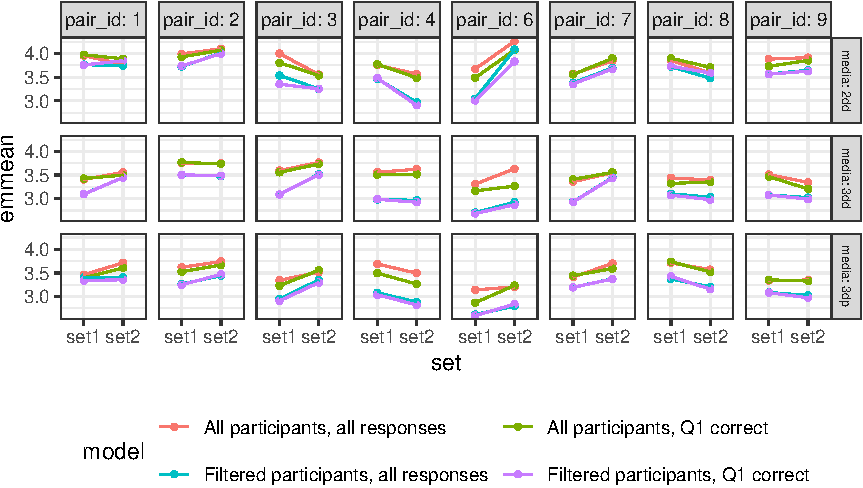
\includegraphics{index_files/figure-pdf/fig-model-int2-1.pdf}

}

\caption{\label{fig-model-int2}Interaction plots for dataset and
response filtering, facetted by stimuli pair and media type.}

\end{figure}%

\begin{figure}

\centering{

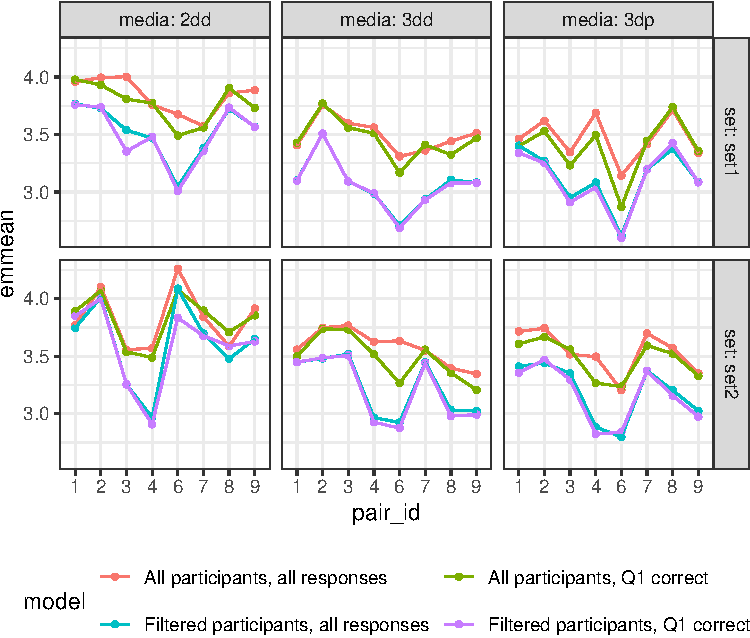
\includegraphics{index_files/figure-pdf/fig-model-int3-1.pdf}

}

\caption{\label{fig-model-int3}Interaction plots for stimuli pairs and
response filtering, facetted by dataset and media type.}

\end{figure}%

\newpage

\begin{tcolorbox}[enhanced jigsaw, toptitle=1mm, leftrule=.75mm, breakable, arc=.35mm, colback=white, colbacktitle=quarto-callout-note-color!10!white, toprule=.15mm, title=\textcolor{quarto-callout-note-color}{\faInfo}\hspace{0.5em}{Note}, titlerule=0mm, colframe=quarto-callout-note-color-frame, coltitle=black, bottomtitle=1mm, opacitybacktitle=0.6, opacityback=0, rightrule=.15mm, bottomrule=.15mm, left=2mm]

This paragraph is pushed to a new page since the ANOVA table p-values is
causing formatting issues

\end{tcolorbox}

Visualizations of the simple effects for media types, datasets, and
stimuli pairs (Figure~\ref{fig-model-int1}, Figure~\ref{fig-model-int2},
Figure~\ref{fig-model-int3}) shows that the difference between
participant filtering is mostly a linear shift in log error. Removing
participants deemed to be random guessers tended to have smaller errors
than including all participants. The shift is less prevalent across
participant filters when filtering out incorrect responses to the first
question in each trial. This, in addition to the p-values from
\textbf{?@tbl-all-models-anova}, suggests that our sample size was large
enough to counteract effects from careless respondents.

We also attempted to fit Gaussian mixture models to the submitted
responses using the \texttt{flexmix} package (Grün and Leisch 2007) to
account for careless respondents (Jaso, Kraus, and Heller 2021).
However, these models only reliably detected a small subset of
participants who were would be considered high performers. That is,
participants who had a near 1:1 relationship with the ratio estimations
strategy and small variation. Visual inspections of the mixture model
components did not provide reliable classifications of estimation
strategies, so we opted to exclude mixture models from consideration.

\subsubsection{Generalized Additive
Model}\label{generalized-additive-model}

In addition to our parametric methods, we also present the results of a
generalized additive model (Hastie 2017). Here, we define the model
similarly to the parametric models, but replace stimuli pair identifiers
with their respective numerical ratio value. Thin-plate regression
splines in the generalized additive model account for nonlinearity which
could alleviate issues due to different estimation strategies. The
formal statistical model is as follows:

\begin{equation}\phantomsection\label{eq-gam}{
y=\mu+S_i\times M_j + s_i^S(R)+s_j^M(R)+P_m+\epsilon
}\end{equation}

where

\begin{itemize}
\item
  \(y=\log_2(|\text{Error}|+1/8)\)
\item
  \(S_i\times M_j\) is the fixed effects for main effect and two-way
  interactions of dataset \(S_i\) and media type \(M_j\)
\item
  \(S_i^S(R)\) is a thin-plate spline function for ratio accounting for
  dataset
\item
  \(S_j^M(R)\) is a thin-plate spline function for ratio accounting for
  media type
\item
  \(P_m\) is the random effect of the \(m^{th}\) participant
\item
  \(\epsilon\) is random error
\end{itemize}

A generalized additive model was fit using the \texttt{mgcv} package
(Wood 2017) on the entire dataset and the filtered dataset. The data for
these models remove stimuli pair 5 and incorrect responses to the
initial question. In both cases, results of the generalized additive
models suggest that the 2D heatmaps have larger errors than the 3D
heatmaps, with no differences detected between the digital and physical
heatmaps \textbf{?@tbl-gam-emmeans}\textbf{?@tbl-gam-diffs}.

\begin{longtable}[]{@{}lrrrr@{}}
\caption{Parametric coefficients in gam model with all
participants.}\tabularnewline
\toprule\noalign{}
& Estimate & Std. Error & t value &
Pr(\textgreater\textbar t\textbar) \\
\midrule\noalign{}
\endfirsthead
\toprule\noalign{}
& Estimate & Std. Error & t value &
Pr(\textgreater\textbar t\textbar) \\
\midrule\noalign{}
\endhead
\bottomrule\noalign{}
\endlastfoot
(Intercept) & 3.773 & 0.083 & 45.613 & 0.000 \\
setset2 & 0.014 & 0.080 & 0.172 & 0.863 \\
media3dd & -0.317 & 0.077 & -4.094 & 0.000 \\
media3dp & -0.389 & 0.089 & -4.359 & 0.000 \\
setset2:media3dd & 0.018 & 0.110 & 0.163 & 0.871 \\
setset2:media3dp & 0.078 & 0.124 & 0.630 & 0.529 \\
\end{longtable}

\begin{longtable}[]{@{}lrrrr@{}}
\caption{Approximate significance of smooth terms in gam mode with all
participants.}\tabularnewline
\toprule\noalign{}
Smooth & edf & Ref.df & F & p-value \\
\midrule\noalign{}
\endfirsthead
\toprule\noalign{}
Smooth & edf & Ref.df & F & p-value \\
\midrule\noalign{}
\endhead
\bottomrule\noalign{}
\endlastfoot
s(target\_ratio):media2dd & 1.002 & 1.003 & 0.058 & 0.813 \\
s(target\_ratio):media3dd & 1.972 & 2.350 & 1.476 & 0.200 \\
s(target\_ratio):media3dp & 1.047 & 1.428 & 1.612 & 0.268 \\
s(target\_ratio):setset1 & 1.005 & 1.009 & 0.650 & 0.422 \\
s(target\_ratio):setset2 & 1.022 & 1.042 & 0.165 & 0.719 \\
s(user\_id) & 217.826 & 258.000 & 6.423 & 0.000 \\
\end{longtable}

\begin{longtable}[]{@{}lrrrr@{}}
\caption{Parametric coefficients in gam model without random
guessers.}\tabularnewline
\toprule\noalign{}
& Estimate & Std. Error & t value &
Pr(\textgreater\textbar t\textbar) \\
\midrule\noalign{}
\endfirsthead
\toprule\noalign{}
& Estimate & Std. Error & t value &
Pr(\textgreater\textbar t\textbar) \\
\midrule\noalign{}
\endhead
\bottomrule\noalign{}
\endlastfoot
(Intercept) & 3.773 & 0.083 & 45.613 & 0.000 \\
setset2 & 0.014 & 0.080 & 0.172 & 0.863 \\
media3dd & -0.317 & 0.077 & -4.094 & 0.000 \\
media3dp & -0.389 & 0.089 & -4.359 & 0.000 \\
setset2:media3dd & 0.018 & 0.110 & 0.163 & 0.871 \\
setset2:media3dp & 0.078 & 0.124 & 0.630 & 0.529 \\
\end{longtable}

\begin{longtable}[]{@{}lrrrr@{}}
\caption{Approximate significance of smooth terms in gam model without
random guessers.}\tabularnewline
\toprule\noalign{}
Smooth & edf & Ref.df & F & p-value \\
\midrule\noalign{}
\endfirsthead
\toprule\noalign{}
Smooth & edf & Ref.df & F & p-value \\
\midrule\noalign{}
\endhead
\bottomrule\noalign{}
\endlastfoot
s(target\_ratio):media2dd & 1.002 & 1.003 & 0.058 & 0.813 \\
s(target\_ratio):media3dd & 1.972 & 2.350 & 1.476 & 0.200 \\
s(target\_ratio):media3dp & 1.047 & 1.428 & 1.612 & 0.268 \\
s(target\_ratio):setset1 & 1.005 & 1.009 & 0.650 & 0.422 \\
s(target\_ratio):setset2 & 1.022 & 1.042 & 0.165 & 0.719 \\
s(user\_id) & 217.826 & 258.000 & 6.423 & 0.000 \\
\end{longtable}

\begin{table}

\caption{Estimated marginal means for generalized additive model}
\centering
\begin{tabular}[t]{llrrrrr}
\toprule
Data filtering & set & emmean & SE & df & lower.CL & upper.CL\\
\midrule
 &  & 3.773 & 0.083 &  & 3.611 & 3.936\\
\cmidrule{3-4}
\cmidrule{6-7}
 &  & 3.532 & 0.090 &  & 3.356 & 3.709\\
\cmidrule{3-4}
\cmidrule{6-7}
 & \multirow{-3}{*}[1\dimexpr\aboverulesep+\belowrulesep+\cmidrulewidth]{\raggedright\arraybackslash set1} & 3.493 & 0.105 &  & 3.286 & 3.700\\
\cmidrule{2-4}
\cmidrule{6-7}
 &  & 3.788 & 0.083 &  & 3.625 & 3.951\\
\cmidrule{3-4}
\cmidrule{6-7}
 &  & 3.565 & 0.091 &  & 3.387 & 3.742\\
\cmidrule{3-4}
\cmidrule{6-7}
\multirow{-6}{*}[2.5\dimexpr\aboverulesep+\belowrulesep+\cmidrulewidth]{\raggedright\arraybackslash All participants} & \multirow{-3}{*}[1\dimexpr\aboverulesep+\belowrulesep+\cmidrulewidth]{\raggedright\arraybackslash set2} & 3.586 & 0.106 & \multirow{-6}{*}[2.5\dimexpr\aboverulesep+\belowrulesep+\cmidrulewidth]{\raggedleft\arraybackslash 3729.128} &  & 3.794\\
\cmidrule{1-5}
\cmidrule{7-7}
 &  & 3.593 & 0.109 &  & \multirow{-2}{*}[0.5\dimexpr\aboverulesep+\belowrulesep+\cmidrulewidth]{\raggedleft\arraybackslash 3.378} & 3.807\\
\cmidrule{3-4}
\cmidrule{6-7}
 &  & 3.150 & 0.107 &  & 2.939 & 3.360\\
\cmidrule{3-4}
\cmidrule{6-7}
 & \multirow{-3}{*}[1\dimexpr\aboverulesep+\belowrulesep+\cmidrulewidth]{\raggedright\arraybackslash set1} & 3.199 & 0.115 &  & 2.973 & 3.425\\
\cmidrule{2-4}
\cmidrule{6-7}
 &  & 3.693 & 0.109 &  & 3.479 & 3.906\\
\cmidrule{3-4}
\cmidrule{6-7}
 &  & 3.361 & 0.108 &  & 3.149 & 3.574\\
\cmidrule{3-4}
\cmidrule{6-7}
\multirow{-6}{*}[2.5\dimexpr\aboverulesep+\belowrulesep+\cmidrulewidth]{\raggedright\arraybackslash Random guessers removed} & \multirow{-3}{*}[1\dimexpr\aboverulesep+\belowrulesep+\cmidrulewidth]{\raggedright\arraybackslash set2} & 3.310 & 0.116 & \multirow{-6}{*}[2.5\dimexpr\aboverulesep+\belowrulesep+\cmidrulewidth]{\raggedleft\arraybackslash 2814.776} & 3.081 & 3.538\\
\bottomrule
\end{tabular}
\end{table}

\begin{table}

\caption{Pairwise differences for generalized additive model}
\centering
\begin{tabular}[t]{lllrrrrr}
\toprule
Data filtering & set & contrast & estimate & SE & df & t.ratio & p.value\\
\midrule
 &  & 2dd - 3dd & 0.241 & 0.088 &  & 2.736 & 0.017\\
\cmidrule{3-5}
\cmidrule{7-8}
 &  & 2dd - 3dp & 0.280 & 0.103 &  & 2.711 & 0.018\\
\cmidrule{3-5}
\cmidrule{7-8}
 & \multirow{-3}{*}[1\dimexpr\aboverulesep+\belowrulesep+\cmidrulewidth]{\raggedright\arraybackslash set1} & 3dd - 3dp & 0.039 & 0.109 &  & 0.361 & 0.931\\
\cmidrule{2-5}
\cmidrule{7-8}
 &  & 2dd - 3dd & 0.223 & 0.089 &  & 2.516 & 0.032\\
\cmidrule{3-5}
\cmidrule{7-8}
 &  & 2dd - 3dp & 0.202 & 0.104 &  & 1.940 & 0.128\\
\cmidrule{3-5}
\cmidrule{7-8}
\multirow{-6}{*}[2.5\dimexpr\aboverulesep+\belowrulesep+\cmidrulewidth]{\raggedright\arraybackslash All participants} & \multirow{-3}{*}[1\dimexpr\aboverulesep+\belowrulesep+\cmidrulewidth]{\raggedright\arraybackslash set2} & 3dd - 3dp & -0.021 & 0.110 & \multirow{-6}{*}[2.5\dimexpr\aboverulesep+\belowrulesep+\cmidrulewidth]{\raggedleft\arraybackslash 3729.128} & -0.192 & 0.980\\
\cmidrule{1-8}
 &  & 2dd - 3dd & 0.443 & 0.091 &  & 4.868 & \\
\cmidrule{3-5}
\cmidrule{7-7}
 &  & 2dd - 3dp & 0.394 & 0.100 &  & 3.925 & \multirow{-2}{*}{\raggedleft\arraybackslash 0.000}\\
\cmidrule{3-5}
\cmidrule{7-8}
 & \multirow{-3}{*}[1\dimexpr\aboverulesep+\belowrulesep+\cmidrulewidth]{\raggedright\arraybackslash set1} & 3dd - 3dp & -0.049 & 0.099 &  & -0.499 & 0.872\\
\cmidrule{2-5}
\cmidrule{7-8}
 &  & 2dd - 3dd & 0.331 & 0.092 &  & 3.585 & \\
\cmidrule{3-5}
\cmidrule{7-7}
 &  & 2dd - 3dp & 0.383 & 0.102 &  & 3.757 & \multirow{-2}{*}{\raggedleft\arraybackslash 0.001}\\
\cmidrule{3-5}
\cmidrule{7-8}
\multirow{-6}{*}[2.5\dimexpr\aboverulesep+\belowrulesep+\cmidrulewidth]{\raggedright\arraybackslash Random guessers removed} & \multirow{-3}{*}[1\dimexpr\aboverulesep+\belowrulesep+\cmidrulewidth]{\raggedright\arraybackslash set2} & 3dd - 3dp & 0.052 & 0.100 & \multirow{-6}{*}[2.5\dimexpr\aboverulesep+\belowrulesep+\cmidrulewidth]{\raggedleft\arraybackslash 2814.776} & 0.521 & 0.861\\
\bottomrule
\end{tabular}
\end{table}

\newpage

\subsection{References}\label{references}

\phantomsection\label{refs}
\begin{CSLReferences}{1}{0}
\bibitem[\citeproctext]{ref-barfield1989}
Barfield, Woodrow, and Robert Robless. 1989. {``The Effects of Two- or
Three-Dimensional Graphics on the Problem-Solving Performance of
Experienced and Novice Decision Makers.''} \emph{Behaviour \&
Information Technology} 8 (5): 369--85.
\url{https://doi.org/10.1080/01449298908914567}.

\bibitem[\citeproctext]{ref-shiny}
Chang, Winston, Joe Cheng, JJ Allaire, Carson Sievert, Barret Schloerke,
Yihui Xie, Jeff Allen, Jonathan McPherson, Alan Dipert, and Barbara
Borges. 2024. {``Shiny: Web Application Framework for r.''}
\url{https://shiny.posit.co/}.

\bibitem[\citeproctext]{ref-cleveland1984}
Cleveland, William S., and Robert McGill. 1984. {``Graphical Perception:
Theory, Experimentation, and Application to the Development of Graphical
Methods.''} \emph{Journal of the American Statistical Association} 79
(387): 531--54. \url{https://doi.org/10.1080/01621459.1984.10478080}.

\bibitem[\citeproctext]{ref-croxton1927}
Croxton, Frederick E., and Roy E. Stryker. 1927. {``Bar Charts Versus
Circle Diagrams.''} \emph{Journal of the American Statistical
Association} 22 (160): 473--82. \url{https://doi.org/10.2307/2276829}.

\bibitem[\citeproctext]{ref-eells1926}
Eells, Walter Crosby. 1926. {``The Relative Merits of Circles and Bars
for Representing Component Parts.''} \emph{Journal of the American
Statistical Association} 21 (154): 119--32.
\url{https://doi.org/10.1080/01621459.1926.10502165}.

\bibitem[\citeproctext]{ref-fischer2000}
Fischer, Martin H. 2000. {``Do Irrelevant Depth Cues Affect the
Comprehension of Bar Graphs?''} \emph{Applied Cognitive Psychology} 14
(2): 151--62.
\url{https://doi.org/10.1002/(SICI)1099-0720(200003/04)14:2\%3C151::AID-ACP629\%3E3.0.CO;2-Z}.

\bibitem[\citeproctext]{ref-fisher1997}
Fisher, Samuel H., John V. Dempsey, and Robert T. Marousky. 1997.
{``Data Visualization: Preference and Use of Two-Dimensional and
Three-Dimensional Graphs.''} \emph{Social Science Computer Review} 15
(3): 256--63. \url{https://doi.org/10.1177/089443939701500303}.

\bibitem[\citeproctext]{ref-flexmix}
Grün, Bettina, and Friedrich Leisch. 2007. {``Fitting Finite Mixtures of
Generalized Linear Regressions in {R}.''} \emph{Computational Statistics
\& Data Analysis} 51 (11): 5247--52.
\url{https://doi.org/10.1016/j.csda.2006.08.014}.

\bibitem[\citeproctext]{ref-hastie2017generalized}
Hastie, Trevor J. 2017. {``Generalized Additive Models.''} In
\emph{Statistical Models in s}, 249--307. Routledge.

\bibitem[\citeproctext]{ref-rlang}
Henry, Lionel, and Hadley Wickham. 2025. {``Rlang: Functions for Base
Types and Core r and 'Tidyverse' Features.''}
\url{https://rlang.r-lib.org}.

\bibitem[\citeproctext]{ref-herzog1981}
Herzog, A. Regula, and Jerald G. Bachman. 1981. {``Effects of
Questionnaire Length on Response Quality.''} \emph{The Public Opinion
Quarterly} 45 (4): 549--59. \url{https://www.jstor.org/stable/2748903}.

\bibitem[\citeproctext]{ref-hofmann2012}
Hofmann, Heike, Lendie Follett, Mahbubul Majumder, and Dianne Cook.
2012. {``Graphical Tests for Power Comparison of Competing Designs.''}
\emph{IEEE Transactions on Visualization and Computer Graphics} 18 (12):
2441--48. \url{https://doi.org/10.1109/TVCG.2012.230}.

\bibitem[\citeproctext]{ref-holloway2019}
Holloway, Leona, Kim Marriott, Matthew Butler, and Samuel Reinders.
2019. {``ASSETS '19: The 21st International ACM SIGACCESS Conference on
Computers and Accessibility.''} In, 183--95. Pittsburgh PA USA: ACM.
\url{https://doi.org/10.1145/3308561.3353790}.

\bibitem[\citeproctext]{ref-multcomp}
Hothorn, Torsten, Frank Bretz, and Peter Westfall. 2008. {``Simultaneous
Inference in General Parametric Models.''} \emph{Biometrical Journal} 50
(3): 346--63.

\bibitem[\citeproctext]{ref-huExploringNewParadigms2015b}
Hu, Michele. 2015. {``Exploring {New Paradigms} for {Accessible 3D
Printed Graphs}.''} In \emph{Proceedings of the 17th {International ACM
SIGACCESS Conference} on {Computers} \& {Accessibility} - {ASSETS} '15},
365--66. Lisbon, Portugal: ACM Press.
\url{https://doi.org/10.1145/2700648.2811330}.

\bibitem[\citeproctext]{ref-huronMakingDataPhysical2023}
Huron, Samuel, Till Nagel, Lora Oehlberg, and Wesley Willett, eds. 2023.
\emph{Making with Data: Physical Design and Craft in a Data- Driven
World}. First edition. {AK Peters} Visualization Series. Boca Raton: AK
Peters : CRC Press.

\bibitem[\citeproctext]{ref-jansen2013}
Jansen, Yvonne, Pierre Dragicevic, and Jean-Daniel Fekete. 2013.
{``Evaluating the Efficiency of Physical Visualizations.''} In
\emph{Proceedings of the {SIGCHI Conference} on {Human Factors} in
{Computing Systems}}, 2593--2602. Paris France: ACM.
\url{https://doi.org/10.1145/2470654.2481359}.

\bibitem[\citeproctext]{ref-jasoIdentificationCarelessResponding2021}
Jaso, Brittany A., Noah I. Kraus, and Aaron S. Heller. 2021.
{``Identification of Careless Responding in Ecological Momentary
Assessment Research: {From} Posthoc Analyses to Real-Time Data
Monitoring.''} \emph{Psychological Methods}, September.
\url{https://doi.org/10.1037/met0000312}.

\bibitem[\citeproctext]{ref-katsioloudis2018}
Katsioloudis, Petros, and Mildred Jones. 2018. {``A Comparative Analysis
of Holographic, 3D-Printed, and Computer-Generated Models: Implications
for Engineering Technology Students{'} Spatial Visualization Ability.''}
\emph{Journal of Technology Education} 29 (2): 36--53.
\url{https://doi.org/10.21061/jte.v29i2.a.3}.

\bibitem[\citeproctext]{ref-kingdom2016}
Kingdom, Frederick A. A., and Nicolaas Prins. 2016. \emph{Psychophysics:
A Practical Introduction}. Second edition. Amsterdam: Elsevier/Academic
Press.

\bibitem[\citeproctext]{ref-kintelOpenSCADDocumentation2023}
Kintel, Marius. 2023. {``{OpenSCAD}. {OpenSCAD}.org.''} July 17, 2023.
\url{http://openscad.org/documentation.html}.

\bibitem[\citeproctext]{ref-kraus2020}
Kraus, Matthias, Katrin Angerbauer, Juri Buchmüller, Daniel Schweitzer,
Daniel A. Keim, Michael Sedlmair, and Johannes Fuchs. 2020. {``CHI '20:
CHI Conference on Human Factors in Computing Systems.''} In, 1--14.
Honolulu HI USA: ACM. \url{https://doi.org/10.1145/3313831.3376675}.

\bibitem[\citeproctext]{ref-spence1989}
Lewandowsky, Stephan, and Ian Spence. 1989. {``The Perception of
Statistical Graphs.''} \emph{Sociological Methods \& Research - SOCIOL
METHOD RES} 18 (November): 200--242.
\url{https://doi.org/10.1177/0049124189018002002}.

\bibitem[\citeproctext]{ref-luModelingJustNoticeable2022}
Lu, Min, Joel Lanir, Chufeng Wang, Yucong Yao, Wen Zhang, Oliver
Deussen, and Hui Huang. 2022. {``Modeling {Just Noticeable Differences}
in {Charts}.''} \emph{IEEE Transactions on Visualization and Computer
Graphics} 28 (1): 718--26.
\url{https://doi.org/10.1109/TVCG.2021.3114874}.

\bibitem[\citeproctext]{ref-mandal2020}
Mandal, B. N., Rajender Parsad, and Sukanta Dash. 2020. {``Incomplete
Split-Plot Designs: Construction and Analysis.''} \emph{Statistics \&
Probability Letters} 166 (November): 108869.
\url{https://doi.org/10.1016/j.spl.2020.108869}.

\bibitem[\citeproctext]{ref-rayshader}
Morgan-Wall, Tyler. 2024. \emph{Rayshader: Create Maps and Visualize
Data in 2D and 3D}.
\url{https://doi.org/10.32614/CRAN.package.rayshader}.

\bibitem[\citeproctext]{ref-muff2022}
Muff, Julian Louis, Tobias Heye, Florian Markus Thieringer, and Philipp
Brantner. 2022. {``Clinical Acceptance of Advanced Visualization
Methods: A Comparison Study of 3D-Print, Virtual Reality Glasses, and
3D-Display.''} \emph{3D Printing in Medicine} 8 (January): 5.
\url{https://doi.org/10.1186/s41205-022-00133-z}.

\bibitem[\citeproctext]{ref-rgl}
Murdoch, Duncan, and Daniel Adler. 2023. \emph{Rgl: 3D Visualization
Using OpenGL}.

\bibitem[\citeproctext]{ref-stevens1986}
Stevens, S. S., and Geraldine Stevens. 1986. \emph{Psychophysics:
Introduction to Its Perceptual, Neural, and Social Prospects}. New
Brunswick, U.S.A: Transaction Books.

\bibitem[\citeproctext]{ref-stusakIfYourMind2016}
Stusak, Simon, Moritz Hobe, and Andreas Butz. 2016. {``If {Your Mind Can
Grasp It}, {Your Hands Will Help}.''} In \emph{Proceedings of the {TEI}
'16: {Tenth International Conference} on {Tangible}, {Embedded}, and
{Embodied Interaction}}, 92--99. Eindhoven Netherlands: ACM.
\url{https://doi.org/10.1145/2839462.2839476}.

\bibitem[\citeproctext]{ref-stusak2015}
Stusak, Simon, Jeannette Schwarz, and Andreas Butz. 2015. {``Evaluating
the {Memorability} of {Physical Visualizations}.''} In \emph{Proceedings
of the 33rd {Annual ACM Conference} on {Human Factors} in {Computing
Systems}}, 3247--50. Seoul Republic of Korea: ACM.
\url{https://doi.org/10.1145/2702123.2702248}.

\bibitem[\citeproctext]{ref-tarr2001}
Tarr, Michael J, and David J Kriegman. 2001. {``What Defines a View?''}
\emph{Vision Research} 41 (15): 1981--2004.
\url{https://doi.org/10.1016/S0042-6989(01)00024-4}.

\bibitem[\citeproctext]{ref-tukey1965}
Tukey, John W. 1965. {``The Technical Tools of Statistics.''} \emph{The
American Statistician} 19 (2): 23--28.
\url{https://doi.org/10.2307/2682374}.

\bibitem[\citeproctext]{ref-vanderplas2020}
Vanderplas, Susan, Dianne Cook, and Heike Hofmann. 2020. {``Testing
Statistical Charts: What Makes a Good Graph?''} \emph{Annual Review of
Statistics and Its Application} 7 (1): 61--88.
\url{https://doi.org/10.1146/annurev-statistics-031219-041252}.

\bibitem[\citeproctext]{ref-vanderplasSignsSineIllusion2015}
VanderPlas, Susan, and Heike Hofmann. 2015. {``Signs of the {Sine
Illusion}---{Why We Need} to {Care}.''} \emph{Journal of Computational
and Graphical Statistics} 24 (4): 1170--90.
\url{https://doi.org/10.1080/10618600.2014.951547}.

\bibitem[\citeproctext]{ref-veit}
Veit, Clairice T. 1978. {``Ratio and Subtractive Processes in
Psychophysical Judgment.''}

\bibitem[\citeproctext]{ref-wang2022}
Wang, Xiyao, Lonni Besançon, Mehdi Ammi, and Tobias Isenberg. 2022.
{``Understanding Differences Between Combinations of 2D and 3D Input and
Output Devices for 3D Data Visualization.''} \emph{International Journal
of Human-Computer Studies} 163 (July): 102820.
\url{https://doi.org/10.1016/j.ijhcs.2022.102820}.

\bibitem[\citeproctext]{ref-ward2023}
Ward, M. K., and Adam W. Meade. 2023. {``Dealing with {Careless
Responding} in {Survey Data}: {Prevention}, {Identification}, and
{Recommended Best Practices}.''} \emph{Annual Review of Psychology} 74
(1): 577--96. \url{https://doi.org/10.1146/annurev-psych-040422-045007}.

\bibitem[\citeproctext]{ref-ggplot2}
Wickham, Hadley. 2016. {``Ggplot2: Elegant Graphics for Data
Analysis.''} \url{https://ggplot2.tidyverse.org}.

\bibitem[\citeproctext]{ref-mgcv}
Wood, S. N. 2017. \emph{Generalized {A}dditive {M}odels: An Introduction
with {R}}. 2nd ed. Chapman; Hall/CRC.

\bibitem[\citeproctext]{ref-zacks1998}
Zacks, Jeff, Ellen Levy, Barbara Tversky, and Diane J. Schiano. 1998.
{``Reading Bar Graphs: Effects of Extraneous Depth Cues and Graphical
Context.''} \emph{Journal of Experimental Psychology: Applied} 4 (2):
119--38. \url{https://doi.org/10.1037/1076-898X.4.2.119}.

\bibitem[\citeproctext]{ref-zhangJustNoticeableDifference2023}
Zhang, Zhao, Xiwu Shang, Guoping Li, and Guozhong Wang. 2023. {``Just
{Noticeable Difference Model} for {Images} with {Color Sensitivity}.''}
\emph{Sensors (Basel, Switzerland)} 23 (5): 2634.
\url{https://doi.org/10.3390/s23052634}.

\end{CSLReferences}




\end{document}
